\documentclass{llncs}
\usepackage{llncsdoc}
\usepackage[utf8]{inputenc}
\usepackage[compatibility=false]{caption}
\usepackage{amsmath}
\usepackage{amsfonts}
\usepackage{amssymb}
\usepackage{bbm}
\usepackage[ruled,vlined,linesnumbered]{algorithm2e}
\usepackage{graphicx}
\usepackage{caption}
\usepackage{subcaption}
\usepackage{graphicx}
\usepackage{dsfont}
\setcounter{secnumdepth}{5}

\author{Amit Wolfenfeld\inst{1}}
\institute{Technion}
\title{Title}

\begin{document}
\maketitle

\begin{abstract}
In machine learning, the notion of multi-armed bandits refers
to a class of online learning problems, in which a learner (also called decision maker or agent) explores and exploits a given set of choice alternatives in the course of a sequential decision process. 
In the standard setting, the learners learns from stochastic feedback in the form of real-valued rewards.

The Dueling Bandits setting is an online learning framework in which actions are restricted to stochastic comparisons between pairs of arms.
It models settings were absolute rewards are difficult to estimate but pairwise preferences are readily available. 

In this paper we propose several new methods for the Dueling Bandit Problem. Our approach extends the Doubler and Sparring algorithm proposed on [???]. We show empirical results using real data from Microsoft Research's LETOR project.
\end{abstract}

\section{Introduction}
	Multi-armed bandit (MAB) algorithms have received considerable attention and have been studied quite intensely in machine learning since the 50's when  Lai and Robbins released their paper [?]. 
	The huge interest in this topic is not very surprising, due to the fact that this MAB setting is not only theoretically challenging but also extremely useful, as can be seen from its use in a wide range of applications. MAB algorithms are used today for solving many problems such as - in search engines [?], online advertisement [?], and recommendation systems [?].
	The multi-armed bandit problem, or bandit problem for short, is one of the simplest instances of the sequential decision making problem, in which a learner needs to select options from a given set of alternatives repeatedly in an online manner -  the name comes from the gambling world in which a gambler decides from a row of slot machines (sometimes known as "one-armed bandits") and decides which machines to play, how many times to play each machine and in which order to play them. When played, each machine provides a random reward from a distribution specific to that machine. 
	The objective of the gambler is to maximize the sum of rewards earned through a sequence of lever pulls. 
	To be more precise, the learner selects one option at a time and observes a numerical (and typically stochastic) reward, providing information on the quality of that arm. The goal of the learner is to optimize an evaluation criterion such as the error rate (the expected percentage of playing a suboptimal arm) or the cumulative regret (the expected difference between the sum of the rewards actually obtained and the sum of rewards that could have been obtained by playing the best arm in each round).
	In order to minimize the regret, the learner has to face the crucial tradeoff at each trial between "exploitation" of the machine that has the apparent highest expected payoff and "exploration" to get more information about the expected payoffs of the other machines. 
	The learner has to find the best "ratio" between playing the arms that produced high rewards in the past (exploitation) and trying other, possibly even better arms the (expected) reward of which is not precisely known so far (exploration).
	There are many variations of the MAB problem and in most of the we assume a numerical reward such as "arm  number 1 has the value of 0.7", however there are many applications where such assumption does not hold,  were the feedback is a pairwise comparison "arm number 1 is better than arm number 2" as opposed to standard bandits.
	There are many cases in the world of machine learning where precise feedback is not available, and only preference feedback is available. In these cases weakly supervised learning and preference learning must be used, and this is what we study here.  		 
	In preference learning, feedback is typically represented in a purely qualitative way, namely in terms of pairwise comparisons or rankings. 
	Feedback of this kind can be useful in online learning, too, as has been shown in online information retrieval.
	Web search and internet marketing are two examples that show the importance for the Dueling Bandits setting. A search engine needs to give the user the best result for his or her query. For every query the search engine lets the user select from several options of search results and receives the feedback according to the users choice. This feedback comes in the form of "the first result is preferred over the other results".  
	Another example is when an advertiser aims to sell products online. The advertiser will direct users to his sale page. 
	Every advertiser wants sell as much as possible therefore they will want to improve their sale page. In order to improve their sale page the advertiser will create several versions of the pages, split the users between them, and see which one is the top performer. This process is called A/B testing, and each page version is represented by an arm in the Multi Armed Bandit  setting. 
	The problem with standard bandits is that there are trends in the market that temporarily decrease or increase the overall performance (Christmas time for instance). 
	Assuming that the arm's order of performance stays the same, meaning the best arm, performance-wise, stays first, the second best arm stays second and so on - Dueling Bandits Algorithms can be used to increase the advertiser's sale performance while keeping the regret to a minimum.	
	Extending the multi-armed bandit setting to the case of preference-based feedback, i.e., the case in which the online learner is allowed to compare arms in a qualitative way, is therefore a promising idea. 
	Indeed, extensions of that kind have received increasing attention in the recent years. 
	The aim of this paper is to provide a survey of the state-of-the-art in the field of Dueling Bandits Algorithms and present several new algorithms. 
	In section 2 we provide a scientific background for the Dueling Bandits Problem. In section 3 we survey the state-of-the-art algorithms. In section 4 we present a new algorithm that out performs the algorithm described in section 3, In section 5 we present the empirical results.
\newpage

\section{Scientific Background}
	In this section we will go into more detail of what the MAB problem is and more importunately the definition of the Dueling Bandits Problem. 
	We discuss two types of settings, the first - Utility Based Dueling Bandit (UBDB) setting and the second Preference Based Dueling Bandit (PBDB) setting.
	\subsection{Multi Armed Bandits}
	As described in the previous section the multi armed bandit problem is a sequential decision making problem, where a learner explores and exploits a stochastic environment. 
	In this setting, the learner performs actions, referred to as arm pulls. 
	The arms belong to an infinite or finite set $X$. 
	If the set is finite we denote $|X|$ by $K$. 
	Each arm $x \in X$ is associated with a probability distribution over $[0, 1]$, with expectation $\mu_{x}$. 
	Throughout this paper we assume the existence of a unique best arm:
	\begin{equation}\label{eq:regret}
		x^* = argmax_{x \in X}(\mu_{x})
	\end{equation}		
	At each round $t > 0$ the learner "pulls" an arm $x_t \in X$ and acquires a stochastic reward or utility $u_t$, independently of all previous rewards (i.i.d). 
	For each arm $x$ and for all rounds $t \geq 1$,  $n_{x}(t)$ denotes the number of times arm $x$ has been "played".
	In this setup the cumulative regret is defined as following:
	\begin{equation}\label{eq:regret}
		R(T) = \sum_{t=1}^{T} \mu(x^*) - u_t
	\end{equation}
	The cumulative regret shows the difference between the utility the player could have acquired if he played the best arm and the sum of utilities actually acquired.
	
	\subsubsection{UCB Algorithm}	
	The most comonly used algorithm for the MAB setting ,the UCB algorithm, is used to minimize the cumulative regret for finite horizon case. 
	It relies on finding an equal probability upper bound for all arms, as seen in line~\ref{line:ref:UCB}, according to the samples so far, called Upper Confidence Bound (hence the name). 
	The bound for arm $x$ decreases as the number of times it had been sampled so far $n_x$ grows.
	At each round, the sampled arm is the arm that potentially has the highest reward, either because it hadn’t been sampled enough, or because the arm’s average reward has been promising.
	
	The UCB algorithm gives the following guarantees:
	
	
\begin{theorem}\label{thm:UCB}[From \cite{...}]

		Running the UCB algorithm with $|X|=K$, with a finite time horizon of $ T > K$, the expected regret is bounded by $R(T) = \mathcal{O} \left( \left(\sum_{x\in X \backslash x^*} \frac{1}{\Delta_x} \right)\log T \right)$, where $\Delta_x$ is the gap between the best arm $x^*$ and arm $x$.

	\end{theorem}		
	Here we present a variant of UCB that uses an additional parameter $ \beta $ to balance between the exploration and exploitation of the algorithm:
	\begin{figure}[h]
	\IncMargin{1em}
		\begin{algorithm}[H]
		\SetKwInput{KwInput}{Input}
		
		\KwInput{$ X,K=|X|$}
			$ t\leftarrow 1$\\
			$\forall x \in X : \hat{\mu_x} \leftarrow 0$\\
			\BlankLine
			
			\While{$t\leq T $}{
				$x_t\leftarrow argmax_{x\in X} \left(\hat{\mu}_x + \beta \sqrt{\frac{\ln t}{n_x}}\right)$ \label{line:ref:UCB}\\
 				play arm $x_t$ and acquire $u_t$\\
 				update $\hat{\mu}_x$
			}
			\caption{UCB}
		\end{algorithm}
		\caption{UCB Algorithm}\label{algo_UCB}
	\end{figure}

	\subsubsection{Thompson Sampling Algorithm}	
	One of the earliest algorithms, given by W. R. Thompson, dates back to 1933. The basic idea is to choose an arm to play according to its probability of being the best arm.
	The Thompson Sampling algorithm proceeds as follows.
	The algorithm maintains the number of successes and failures for each arm, and holds a random variable with $\beta$-distribution for each arm $\Theta_x\sim Beta(Success_x+1,Failures_x+1)$.
	At each round all the random variables $\Theta_{x,t}$ are sampled.
	The chosen arm is then given by $ x_t \in argmax_{x\in X} \Theta_{x,t}$. 
	While the theoretical behaviour of Thompson sampling has remained elusive for a long time, fairly good understanding of its theoretical properties was achieved by Agrawal and Goyal [?] the first logarithmic regret bound was proved: 
	
	\begin{theorem}\label{thm:TS}[From \cite{...}]

		Running the Thompson Sampling algorithm with $|X|=K$, with a finite time horizon of $ T > K$, the expected regret is bounded by $R(T) = \mathcal{O} \left( \left(\sum_{x\in X \backslash x^*} \frac{1}{\Delta_x^2} \right)^2 \log T \right)$, where $\Delta_x$ is is the gap between the best arm $x^*$ and arm $x$.

	\end{theorem}	
	The pseudo-code of the Thompson Sampling algorithm can be seen in Figure \ref{algo_TS}:
	
	\begin{figure}[h]
	\IncMargin{1em}
		\begin{algorithm}[H]
		\SetKwInput{KwInput}{Input}
		
		\KwInput{$ X,K=|X|$}
			$ t\leftarrow 1$\\
			$\forall x \in X : Success_{x} \leftarrow 0$\\
			$\forall x \in X : Fails_{x} \leftarrow 0$\\			
			\BlankLine
			
			\While{$t\leq T $}{
				$\forall x \in X : \Theta_{x,t} \sim Beta(Success_{x}+1, Fails_{x}+1)$\\
				$x_t\leftarrow argmax(\Theta_{x,t})$\\
 				play arm $x_t$ and acquire $u_t$\\
 				$Success_{x_t} \leftarrow Success_{x_t} + u_t$\\
 				$Fails_{x_t} \leftarrow Fails_{x_t} + (1-u_t)$
			}
			\caption{Thompson Sampling}
		\end{algorithm}
		\caption{Thompson Sampling Algorithm}\label{algo_TS}
	\end{figure}	
	
	\subsection{Dueling Bandits}
		To formalize the problem of learning from preferences, we consider the following interactive online learning model,for the K-armed dueling bandit problem (Yue et al., 2012).
		At each iteration $t$, the learning system presents two arms $x_t, y_t \in X$ to the learner, where $X$ is the set (either finite or infinite) of possible actions. The two arms are compared and the feedback comes in the form of a binary random variable $b_t$, declaring which arm beats the other arm.
		In this paper we will study two different problem settings.
		The first \textbf{UBDB} Utility Based Dueling Bandits, where each arm $x_t$, $y_t$ acquires a utility, unobservable by the learner, and the feedback $b_t$ "behaves" according to the utilities. 
		The second - \textbf{PBDB} - Preference Based Dueling Bandits, where the outcome of the comparison between the arms behaves according to a predefined preference matrix $P$ that characterises the relationship between the arms.
	\subsubsection{UBDB}
		In this setting each of the two arms has an associated random reward (or utility) for the learner, which we denote by $u_t$ and $v_t$, respectively.
		The quantity $u_t$ (resp. $v_t$) is drawn from a distribution that depends on $x_t$ (resp. $y_t$) only.  
		We assume, as always, these utilities are in $[0, 1]$. 
		The learner is rewarded the average utility $ U_{av}(t) = (u_t + v_t)/2$ \footnote{ where \textit{av} is shorthand for average} of the two actions it presents, but it does not observe this reward. 
		Instead, it only observes the a binary choice among the two alternative arms $x_t, y_t$, which depends on the respective utilities $u_t$ and $v_t$. 
		In particular, we model the observed choice as a binary random variable $b_t$ distributed according to:
		\begin{equation}\label{eq:b_t}
		\begin{cases}
		P(b_t = 1|u_t, v_t) = \phi(u_t, v_t)
		\\
		P(b_t = 0|u_t, v_t) = \phi(v_t, u_t)
		\end{cases}
		\end{equation}			
	where $\phi:[0, 1] \times [0, 1] \rightarrow [0, 1]$ is a link function. 
	Clearly, the link function has to satisfy $\phi(A, B) + \phi(B, A) = 1$.
	$b_t$ can be viewed as an indicator for the event $x_t \succ y_t $, or in words "$x_t$ beats $y_t$ in round $t$".
	We assume $u_t$ is drawn from a distribution of expectation $\mu(x_t)$ and $v_t$ independently from a distribution of expectation $\mu(y_t)$.
	The link function $\phi$, which is assumed to be known, quantitatively determines how to translate the utilities $u_t, v_t$ to winning probabilities. 
	The linear link function $\phi_{lin}$ is defined by
	\begin{equation}\label{eq:link_function}
		P(b_t = 1|u_t, v_t) = \phi_{lin}(u_t, v_t) = \frac{1+v_t-u_t}{2}\in [0,1]
	\end{equation}
	For the UBDB case the definition of the regret is very natural and straight forward:

	\begin{equation}\label{eq:utility_regret}
		R_U(T) = \sum_{t=1}^T \mu(x^*)-U_{av}(t)
	\end{equation}	
	Where, as always,  $x^* = argmax_{x \in X} \mu(x)$. 
	This implies that expected zero regret is achievable by setting $(x_t, y_t) = (x^*,x^*)$.
	It should be also clear that playing $(x^*,x^*)$ is pure exploitation, because the feedback is then an unbiased coin with zero exploratory information.
	
	\subsubsection{PBDB}	
		Same as in the UBDB setting	consider a fixed set of arms $X = \{x_1,..,x_k\}$. 
		As actions, the learner performs a comparison between any pair of arms $x_t$ and $y_t$ , meaning the action space is identified with the set of index pairs $(i, j)$ such that $1 \leq i \leq j \leq K$. 
		In this paper we characterise the feedback of the comparison by an unknown preference matrix $P$, which is not necessarily devised from the latent utility.
		More precisely
		
		\begin{equation}\label{eq:preference_matrix}
			P = [p_{x,y}] \in [0,1]^{K \times K} 
		\end{equation}
		To be more precise - for each pair of arms $(x ,y)$, this relation specifies the probability of the event
		\begin{equation}\label{eq:p_xy}
			Pr(x \succeq y) = p_{x, y}
		\end{equation}
		of observing a preference for $x$ in a direct comparison with $y$. 
		Meaning, each $p_{x,y}$ defines a Bernoulli distribution.
		Throughout this paper we assume the these probabilities are independent and stationary during all rounds $t > 0$.		
		This means that whenever two arms is played $(x ,y)$ and compared, the outcome is distributed according to (1), without any dependencies on the previous iterations.
		The relation matrix $P$ is reciprocal in the sense that $p_{x,y} = 1-p_{x,y}$ for all $x,y \in X$.		
		Arm $x$ is said to outperform arm $y$ if $p_{x,y} > 1/2$, meaning the probability of winning in a pairwise comparison is larger for $x$ than it is for $y$ . 
		The closer $p_{x,y}$ is to $1/2$, the harder it is to distinguish between arm $x$ and arm $y$ based on a finite sample set from $Pr(x \succeq y)$. This resembles the case in the standard MAB problem where the gap $\Delta_{x,y}$ is very small.
		 When $p_{x,y} = 1/2$, the learner cannot decide which arm is better based on a finite number of pairwise comparisons.
		 Defining a regret is more tricky in PBDB. In particular, it is necessary to make assumptions on $P$ for the definition to make sense.
		 In (Joachims and Yue, 2011) "Relaxed Stochastic Transitivity" is assumed, defined by:
		 For any triplet of arms $x \succ y \succ z$ and some $ \gamma \geq 1 $, 
		 we assume $\gamma \Delta_{x,z} \geq \max(\Delta_{x,y},\Delta_{y,z})$.
		 Where $\Delta_{x,y}$ is defined
		 \begin{equation}\label{eq:delta}
		 	\Delta_{x,y} = p_{x,y} - 1/2
		 \end{equation}		 		 
		 In a later paper (Urvoy et al., 2013) this assumption was relaxed, and only a Condorcet winner is assumed, where a Condercet winner is defined as an arm $x$, such that $ \forall y, p_{x,y} > 1/2$. 
		 Given a Condorcet winner, we define regret for each time-step as follows (Yue et al., 2012): if arms $x$ and $y$ were chosen for comparison at time $t$, then regret at that time is $ \frac{\Delta_{x^*,x_t}+\Delta_{x^*,y_t}}{2} $ and the cumulative regret is
		 \begin{equation}\label{eq:preference_regret}
		 R_P(T) = \sum_{t=1}^T \frac{\Delta_{x*,x_t}+\Delta_{x*,y_t}}{2}
		 \end{equation}
%		 Where $\Delta_{x,y}$ is defined		 
%		 $$ \Delta_{x,y} = p_{x,y} - 1/2$$
%		 This to be a good quantity to characterize the "damage" that is inflicted for each choice the learner makes during the Dueling Bandits game.
		 As opposed to the standard bandit game $\Delta_{x,y}$ can be negative, in which the quantity used for the multi-armed bandit task is always positive and depends on the gap between the means of the best arm and the suboptimal arms.
		 
	\subsection{Probability Estimation}		 
		The Dueling Bandit game is played in discrete rounds, either through a finite time horizon or an infinite horizon. 
		 As described in the previous section, the learner compares between two arms in each round $t > 0$. 
		 And so, in each round $t$, the learner selects a pair of arms $x_t,y_t$ and observes
	\begin{equation}
		\begin{cases}
    		x_t \succeq y_t & \text{with probablity } p_{x_t,y_t} 
       	\\
    		y_t \succeq x_t & \text{with probablity } p_{y_t,x_t}
	\end{cases}
	\end{equation}		
	In this paper the pairwise probabilities $p_{x,y}$ can is estimated according to the finite sample sets.
	We consider the set of rounds among the first $t$ iterations, in which the learner decides to compare arms $x$ and $y$ , and denote the size of this set by $n_{x,y}$, or the number of times $x$ and $y$ have been compared.  
	We denote the number of times $x$ "beat" over $y$ by $w_{x,y}$ and $w_{y,x}$ the number of "beat" of $y$ over $x$.
	It is easy to see that $n_{x,y} = n_{y,x} = w_{x,y}+w_{y,x}$ and so the unbiased estimation of $p_{x,y}$ up to iteration $t$ is then given by
	\begin{equation}\label{eq:est_pxy}
		\hat{P}_{x, y} = \frac{w_{x,y}}{n_{x,y}} = 
		\frac{w_{x,y}}{w_{x,y}+w_{y,x}}
	\end{equation}	 
	As mention above, in this paper we assume that the samples are independent and identically distributed (i.i.d), $\hat{p}_{i,j}$ is a good estimate of the pairwise probability (2). 
	As in most MAB algorithms a high probability confidence interval is obtained by the Hoeffding bound defined in Theorem~\ref{thm:Hoeffding}. 
	The confidence intervals may differ from one algorithm to another, but usually it is of the form $[p_{x,y} \pm c_{x,y} ]$. 
	According to this definition arm $x$ outperforms arm $y$ with high likelihood if $p_{x,y} + c_{x,y} > 1/2]$, and, $x$ is beaten by arm $y$ with high probability, if $p_{x,y} + c_{x,y} < 1/2]$.
	\subsubsection{Hoeffding Inequality}	
	As a preliminary step, we remind Hoeffding’s inequality.
	\begin{theorem}\label{thm:Hoeffding}[From \cite{...}]
	Suppose $\{X_1,..,X_N \}$ are independent random variables with values in the interval $[a,b]$.
	We denote $\bar{X}_N = \sum_{i=1}^N \frac{X_i}{N}$.\\
	If $E[\bar{X}_N] = \mu_X$, then for any $d>0$:
	\begin{subequations}
	\begin{equation}
	Pr(\bar{X}_N \geq \mu_X+ d) \leq e^{-\frac{2d^2}{(b-a)^2}\cdot\frac{1}{N}}
	\end{equation}
	\begin{equation}
	Pr(\bar{X}_N \leq \mu_X- d) \leq e^{-\frac{2d^2}{(b-a)^2}\cdot\frac{1}{N}}
	\end{equation}
	\end{subequations}
	\end{theorem}
	\subsection{The Relation Between Preference and Utility based Regrets}
	
	In the extreme case where the preference matrix $P$ is induced by \textbf{UBDB} we argue that the regret defined in  section 2.2.1 is the same as in  section 2.2.2. 
	We will show that using the definition of the linear link function both utility based regret and preference based regret are the same (upto a factor of 2): 
	\begin{equation}\label{eq:ref1}
		p_{x^*,y} = \phi_{lin}(\mu(x^*),\mu(y)) = \frac{1 +\mu(y)-\mu(x^*)}{2}
	\end{equation}
	Incorporating \eqref{eq:ref1} in the definition of $\Delta_{x,y}$ we get
	$$
	\Delta_{x^*,y} = p_{x^*,y} - \frac{1}{2} = \frac{\mu(x^*)-\mu(y)}{2}
	$$
	And so the total regret is defined:
	\
	$$ R_P(T) = \sum_{t=1}^T \frac{\Delta_{x^*,x_t}+\Delta_{x^*,y_t}}{2} =  
\sum_{t=1}^T \frac{\frac{\mu(x^*)-\mu(x_t)}{2}+\frac{\mu(x^*)-\mu(y_t)}{2}}{2} =
$$

$$
\frac{1}{2} \sum_{t=1}^T \mu(x^*) -\frac{
	\mu(x_t)+\mu(y_t)}{2} =
\frac{1}{2} \sum_{t=1}^T \mu(x^*)- U_{av} = \frac{1}{2}R_U(T)$$

\subsection{Table of Notations}
For the convenience of the reader we have included a table of all the definitions. 
	\begin{table}[h]
		\begin{tabular}{ll}
 			$T$ & Horizon \\
 			$t$ &  Round \\
 			$X$ & Arms space \\
 			$K = |X|$ & Total Number of Arms\\
 			$x_t \in X$ & Left arm \\
 			$y_t \in X$ & Right arm \\
 			$u_t \in \mu_t$ & Left utility \\
 			$v_t \in \mu_t$ & Right utility \\
 			$b_t$ & Observed feedback \\
 			$R_U(T)$ & Total Utility Based Regret till T\\
			$R_P(T)$ & Total Preference Based Regret till T\\
 			$\mathcal{P}$ & Set of potential arms \\
 			$\hat{P}_{x, y}$ & Estimate of $P(x>y)$\\
 			$\hat{C}_{x, y}$ &   Confidence interval of - $(\hat{P}_{x, y} - \sqrt{log(1/\delta)/t},\hat{P}_{x, y} +\sqrt{log(1/\delta)/t})$\\
 			$n_x$ &   The number of times arm $x$ has been played\\
 			$w_x$ & The number of times arm $x$ has won\\
 			$\hat{P}_x  $ &  $ w_x / n_x $\\
 			$ W = [w_{x,y}]$ & Number of wins of arm $x$ over arm $y$\\
 			$U = [u_{x,y}]$ &  Utility function\\
 			$\Theta_{x,y}$ &   Random variable with Beta distribution.
		\end{tabular}
	\end{table}

\section{Survey of Algorithms for Dueling Bandits}
	We start by surveying dueling bandit algorithms. In this section we have included Interleaved Filtering, Beat the Mean Bandit, RUCB, RCS, SAVAGE and the Sparring and Doubler algorithms for they served as a foundation for our new approach. We categorize these algorithm based on the following criteria - Explore and Exploit algorithms and Pure Exploitation algorithms.

\subsection{Explore and Exploit Algorithms}
	In the finite horizon case most PBDB algorithms are based on the idea of splitting the rounds into two phases, exploration and then exploitation. In the first phase the algorithm identifies the best arm with high probability. In the second phase the algorithm repeatedly compares the chosen arm to itself.
	Such algorithm, using the above principle are called "explore-then-exploit" algorithms.
	The main draw back for these algorithm is that $T$, the horizon, is needed to be known in advance. The horizon is needed for the algorithm to control the trade-off between exploration and exploitation and to control the regret accumulated in the event of failure to identify the best arm.
	To be more specific, let's assume the algorithm can identify the best arm with probability of at least $1-\delta$. We will set $\delta$ to $1/T$ and so the algorithm can guarantee that the best arm is chosen within $T$ rounds with probability greater then $1-1/T$.
	Let's define $R_{explore}(T),R_{exploit}(T)$, the regrets for the exploration phase and exploitation phase, that define the total regret:
	$$R(T) = R_{explore}(T)+R_{exploit}(T)$$
	Assuming the algorithm made a mistake and did not choose the best arm at the end of exploration phase, the regret accumulated , $R_{explore}(T)+R_{exploit}(T)$ is at most $\mathcal{O}(T)$, since the regret accumulated in each round is bounded by 1.
	Assuming the algorithm did choose the best arm $R_{exploit}(T)$ is $0$.
	Consequently, the expected regret of an explore-then-exploit algorithm is
	\begin{equation}
		E[R(T)] \leq (1-1/T)E[R_{explore}(T)] +(1/T)\mathcal{O}(T) = \mathcal{O}(E[R_{explore}(T)]+1)
	\end{equation}
	The same argument holds for the case of high probability regret bounds in the explore-then-exploit framework. 
	In summary, the performance of an explore-then-exploit algorithm is bounded by the performance of the exploration algorithm. 
	Although Explore and Exploit algorithms need to know the Horizon $T$ in advance, by using a simple workaround ,the "Squaring Trick", these algorithm can be used in the infinite horizon setting. An estimated horizon $\hat{T}$ is submitted to the algorithm and once the algorithm reaches $t=\hat{T}$ the horizon is set to $\hat{T}^2$, this process continues till the algorithm terminates, and hence the name "Squaring Trick".
	
	\subsection{Pure Exploration Algorithms}
	In the infinite time horizon case , in which no horizon is specified and the evaluation process continues indefinitely.
	In this case it is not sufficient for the algorithm to maximize accuracy or minimize regret after a single horizon is reached. 
	Instead, it must minimize regret by rapidly decreasing the frequency of comparisons involving suboptimal arms, particularly those that fare worse in comparison to the best arm.
	In the standard bandit problems, the arm that is chosen in each round produces an expected reward that is at most $\epsilon$ shy of the optimal arm, the $\epsilon$-optimal arm.
	In the PBDB case approximation errors are harder to define.  
	A preference-based MAB algorithm is an ($\epsilon, \delta$)-PAC PBDB algorithm with a sample complexity $B(P,\epsilon,\delta)$, if it returns the $\epsilon$-optimal arm with probability at least $1-\delta$ , and the number of comparisons taken by the algorithm is at most $B(P,\epsilon,\delta)$.
	The sample complexity of the learner is then the number of pairwise comparisons it makes before concluding the optimal arm, and the corresponding bound is denoted $B(P,\epsilon,\delta)$ where $P$ is defined at \eqref{eq:preference_matrix}.

	\subsection{The Algorithms}
\subsubsection{Interleaved Filter}
	Yue et al.[?] propose an algorithm for a finite horizon setting. 
	Their algorithm works for the scenario in which the preference matrix satisfies the following properties:

	\begin{enumerate}

		\item Strong stochastic transitivity.

		\item Stochastic triangle inequality

	\end{enumerate}
	Strong stochastic transitivity means that for any triplet of arms $x \succ y \succ z$ we assume $\Delta_{x,z} \geq \max(\Delta_{x,y},\Delta_{y,z})$.
	Stochastic triangle inequality means that for any triplet of arms $x \succ y \succ z$ we assume $\Delta_{x,z} \leq \Delta_{x,y} + \Delta_{y,z}$.
	The regret is defined as in \eqref{eq:preference_regret}.
	The algorithm implements an explore-then-exploit strategy. 
	This means that the time steps $1..T$ are divided into two phases, the first serving for exploration only (learning) and the second for exploitation only. 
	In particular, in the exploitation phase, the algorithm plays only the apparent optimal action consistently.
	The exploration phase works by repeated elimination as follows. 
	At each step the algorithm maintains a working set of arms that are potential optimal. 
	It is shown that with high probability the true optimal arm is consistently in the working set. 
	The elimination is done using a round robin tournament strategy, as shown in line~\ref{lst:line:rr} of algorithm~\ref{algo_IF}. 
	Each arm in the working set is compared against all the arms in the working set, until sufficient confidence is achieved to determine whether the arm must be eliminated (removed from the working set). 
	By sufficient confidence we mean that with high probability an arm cannot be the optimal. This is encoded in the following prediction(line~\ref{lst:line:elimination}):
	 $$p_{x,y}+c_{x,y}<1/2$$
	Apart from the round robin elimination, a pruning process is executed.
	We explain the pruning process more precisely. 
	As can be seen in line~\ref{lst:line:pruning}, an element $y$ is removed from the working set $\cal P$ if $$p_{x,y}-c_{x,y}<1/2$$ 
	In words, this condition implies that $y$ is with high confidence inferior compared to the current candidate in the round robin.
	Once a single arm is left in the working set, the algorithm enters the exploitation phase.
	The algorithm pseudo-code is presented in Figure~\ref{algo_IF}. 
	The guarantee provided is as follows:

	\begin{theorem}\label{thm:IF}[From \cite{...}]

		Running the Interleaved Filter algorithm with $|X|=K$, with a known finite time horizon of $T>K$, the expected regret is bounded by $R_P(T) = \mathcal{O} \left( \frac{K\log K}{\Delta_{x^*,y}} \log T \right)$, where $y$ is an arm that is only beaten by $x^*$.

	\end{theorem}
	From the analysis of the algorithm it can be seen that the algorithm returns the best arm with probability of $1-\frac{1}{T}$.
	Correspondingly, a suboptimal arm is returned by the algorithm with probability of $\frac{1}{T}$ hence , similar to a PAC type argument: With high probability of at least $1-\frac{1}{T}$, the estimated regret after $T$ steps is at most $\mathcal{O} \left( \frac{K\log K}{\Delta^*} \log T \right)$. The regret is defined as in \eqref{eq:preference_regret}.
	
	\begin{figure}[h]
	\IncMargin{1em}
		\begin{algorithm}[H]
		\SetKwInput{KwInput}{Input}
		
		\KwInput{$T$,$ X,K=|X|, \delta$}
			$ t\leftarrow 1$\\
			$ \mathcal{P} \leftarrow X$
			Choose $x_t \in \mathcal{P}$ randomly\\
			$ \mathcal{P} \leftarrow \mathcal{P} \backslash x_t$\\
			\BlankLine
			\While{$|\mathcal{P}|>1 $}{

 				\For{$x \in \mathcal{P}$\label{lst:line:rr}}{
					compare($y, x_t$)\\
					update($\hat{P}_{x_t, y}$)\\
					$t \leftarrow t+1$	
				}
				$c_t \leftarrow \sqrt{log(1/\delta)/t}$\\
				\While{$\exists y \in$ s.t. $\left( \hat{P}_{x_t,y}+c_t<1/2 \right)$\label{lst:line:elimination}}{
				$\mathcal{P} \leftarrow \mathcal{P} \backslash \{y\}$
				}
				\If{$\exists y \in$ s.t. $( \hat{P}_{x_t,y}-c_t <1/2 )$\label{lst:line:pruning}}{
					$x_{t+1} \leftarrow y$\\
					$\mathcal{P} \leftarrow \mathcal{P} \backslash \{ y \}$\\
					$\forall x \in \mathcal{P}$ reset $\hat{P}_{y,x}$
				}
			}
			\Return{$x_t \in \cal P$}
			\caption{Interleaved Filter}
		\end{algorithm}
		\caption{Interleaved Filter Algorithm}\label{algo_IF}
	\end{figure}
	

\subsubsection{Beat The Mean Bandit}
	Yue and Joachims [?] proposed an explore-then-exploit strategy, for a finite horizon setting, very similar to IF. 
	Beat the Mean (BTM) - a preference-based online learning algorithm.
	This algorithm is based on relaxed assumptions with regards to the IF algorithm:
	\begin{enumerate}
		\item Relaxed stochastic transitivity.
		\item Stochastic triangle inequality
	\end{enumerate}
	Relaxed stochastic transitivity means that for any triplet of arms $x \succ y \succ z$ and for some $ \gamma \geq 1 $ we assume $\gamma\Delta_{x,z} \geq  \max(\Delta_{x,y},\Delta_{y,z})$.
	The main idea of BTM is to maintain a score of the "Mean Bandit" (arm in our case) and eliminating arms that are inferior to it with enough confidence.
	Similar to the IF algorithm BTM maintains a working set of potentially optimal arms.
	At each round the algorithm picks an arm that has the least plays in the corresponding current history, $n_x$, and compares it with a randomly chosen arm from the working set.
	Comparing an arm against random arms in the working set is functionally identical to comparing an arm against the "Mean Bandit" sampled uniformly from the working set.
	The arm, $x$,  that is empirically worst arm and is separated enough from the best arm with enough confidence is defined using:
	\begin{equation}\label{eq:BTM_el}
	min_{x\in \mathcal{P}} (\hat{P}_{x})+c^* \leq max_{y \in \mathcal{P}}(\hat{P}_{y})-c^*
\end{equation}	 
	Once an arm reached \eqref{eq:BTM_el} (see line~\ref{alg:BTM:elimination}) it is eliminated from the working set. The confidence is defined as $ c^* = c_{\delta, \gamma}(n^*) $, where $c_{\delta, \gamma}(n) = 3\gamma^2 \sqrt{\frac{1}{n}\log \frac{1}{\delta}}$.
	The algorithm pseudo-code is presented in Figure~\ref{algo_BTM}.	
	The guarantee provided is as follows:
	\begin{theorem}\label{thm:BTM}[From \cite{...}]

		Running the Beat the Mean Bandit algorithm with $|X|=K$, with a known finite time horizon of $T>K$, the expected regret is bounded by $R_P(T) = \mathcal{O} \left( \frac{\gamma^7K}{\Delta_{x^*,y}} \log T \right)$, where $y$ is an arm that is only beaten by $x^*$.

	\end{theorem}	
	Similarly to the analysis of the IF algorithm it can be seen that the algorithm returns the best arm with probability of $1-\frac{1}{T}$.	
	
	\begin{figure}[h]
	\IncMargin{1em}
		\begin{algorithm}[H]
		\SetKwInput{KwInput}{Input}
		
		\KwInput{$T$,$X,K=|X|, c_{\delta, \gamma}(\cdot)$}
			$ \mathcal{P} \leftarrow X $\\
			$ W = [w_{x,y}]$\\
			$ \forall x \in \mathcal{P} , n_x \leftarrow 0 $\\
			$ \forall x \in \mathcal{P} , w_x \leftarrow 0 $\\
			$ \forall x \in \mathcal{P} ,\hat{P}_x \leftarrow w_x / n_x$ or $0$ if $n_x = 0 $\\
			$t \leftarrow 0$ \\
			\BlankLine
			\While{$|\mathcal{P}|>1$}{
				$x_t \leftarrow argmin_{x \in \mathcal{P}} n_x$\\
				select $y_t\in \mathcal{P}$ at random\\
				compare($x_t$, $y_t$)\\
				update($W$)\\
				$n_{x_t} \leftarrow n_{x_t}+1$\\ 
				$ n^*  \leftarrow \min_{x \in \mathcal{P}} n_x$\\
				$ c^* \leftarrow c_{\delta, \gamma}(n^*) $ or $1$ if $ n^* = 0$\\
				\If{$min_{y\in \mathcal{P}} (\hat{P}_{y})+c^* \leq max_{x \in \mathcal{P}}(\hat{P}_{x})-c^*$ \label{alg:BTM:elimination}}{
					$y\leftarrow argmin_{x\in \mathcal{P}}\hat{P}_{x}$\\
					$\forall x \in \mathcal{P}$ delete comparison with $y$ from $w_y, n_y$\\
					$\mathcal{P} \leftarrow \mathcal{P}\backslash\{y\} $\\
				} 
			$t \leftarrow t+1$
			}
			\Return{$x_t \in \cal P$}
			\caption{Beat the Mean Bandit}
		\end{algorithm}
		\caption{Beat the Mean Bandit Algorithm}\label{algo_BTM}
	\end{figure}

	\subsubsection{RUCB} Relative Upper Confidence Bound by Zoghi et al. [?], adapts the most commonly used algorithm UCB [Algorithm~ \ref{algo_UCB}] in the standard MAB setting to the Dueling Bandit setting (PBDB version).
	The algorithm assumes that a Condorcet winner exists.
	A Condorcet winner is a definition borrowed from social choice \cite{work by condorcet}.  Roughly speaking, a Condorcet winner beats all the other arms on average. Mathematically, a Condorcet winner (if exists) is defined by: $x$ is the Condorcet winner if $ p_{x,y} > 1/2, \forall y $.
	The algorithms pseudo-code is presented in Figure~\ref{algo_RUCB}.
	Similarly the the UCB algorithm the RUCB algorithm maintains an upper confidence bound $u_{x_t,y_t}$, for each pair of arms, as seen in line~\ref{alg:rucb:line:ucb_set} of Algorithm~\ref{algo_RUCB}.
	On each round, RUCB selects the arms to compare from the set of potential Condorcet winners, meaning the set of arms for which all are potentially Condorcet winners with sufficiently high probability. 
	After selecting the set of potential Condercet winners the algorithm selects the pair of arms with the highest upper confidence bound $u_{x_t,y_t}$, this can be seen as a Dueling Bandit version of the "optimism in the face of uncertainty" principle from UCB.
	Note that in line~\ref{alg:rucb:line:ucb_choose_set} the comparisons are based on $u_{x_t,y_t}$ and in line~\ref{alg:rucb:line:ucb_choose} of Algorithm~\ref{algo_RUCB} the comparisons are based on $u_{y_t,x_t}$ making it more difficult for the algorithm to compare an arm against itself.
	Thus, RUCB strives to avoid auto-comparisons (comparisons of an item with itself) until there is great certainty that $x_t$ is indeed the Condorcet winner.
	Roughly speaking, if the algorithm would pick the arm $y_t$ according to $u_{x_t,y_t}$ and not $u_{y_t,x_t}$, the algorithm will pick the arm according to the impact of $x_t$ and not $y_t$ and is more likely to pick the pair $x_t,y_t = x_t,x_t$. 
	The RUCB algorithm guarantees the following:
	\begin{theorem}\label{thm:BTM}[From \cite{...}]

		Running the RUCB algorithm with $|X|=K$, with a finite time horizon of $T>K$, the expected regret is bounded by $R_P(T) = \mathcal{O} \left( \frac{K log T}{\Delta_{x^*,y}} \right)$, where $y$ is an arm that is only beaten by $x^*$.

	\end{theorem}
	
	\begin{figure}[h]
	\IncMargin{1em}
		\begin{algorithm}[H]
		\SetKwInput{KwInput}{Input}
		
		\KwInput{$T$,$X,K=|X|, \alpha >1/2,T \in \{1,2,... \}$}
		$ W = [w_{x,y}]$\\
		\BlankLine
		\For{$t =1,2..,T $}{
			$U = [u_{x,y}] \leftarrow \frac{w_{x,y}}{w_{x,y}+w_{y,x}} +\sqrt{\frac{\alpha \cdot \ln(t)}{w_{x,y}+w_{y,x}}}$ \label{alg:rucb:line:ucb_set}\\
			$\forall x \in X : u_{x,x} \leftarrow 0 $\\
			Pick any $x_t$ that satisfies $u_{x_t,x} \geq 1/2, \forall x$. \label{alg:rucb:line:ucb_choose_set}\\
			If no $x_t$ exists pick $x_t$ randomly from $X$.\\
			$y_t \leftarrow argmax_{y} u_{y,x_t}$\label{alg:rucb:line:ucb_choose}\\
			compare($x_t$ , $y_t$)\\
			update($W$) 
} 
			\caption{RUCB}
		\end{algorithm}
		\caption{RUCB Algorithm}\label{algo_RUCB}
	\end{figure}
	
	\newpage
\subsubsection{RCS}
	(Munos et al., 2014) Relative Confidence Sampling is very similar to RUCB in the sense that it aims to minimize cumulative regret and does not eliminate arms from a working set.
	The algorithms pseudo-code is presented in Figure~\ref{algo_RCS}.
	Similarly to the RUCB algorithm, the RCS algorithm's only assumption is the existence of a Condorcet winner.
	
	On each round the algorithm simulates a tournament between all the arms, against all the arms. 
	The simulation is conducted, as seen in line~\ref{alg:rcs:simulation}, according to a random variable $\Theta_{x,y} $	with $Beta(\alpha,\beta)$ distribution. 
	The hyper-parameters, $\alpha,\beta$, are $w_{x,y}+1,w_{y,x}+1$ accordingly. Where $w_{x,y}$ is the number of times arm $x$ beat arm $y$.
	The main idea behind this simulation technique is to use the superior performance of Thompson Sampling [?], in the same manner it is used in the K-armed bandit setting. 
	Once the simulation is over, similarly to the RUCB algorithm, the RCS algorithm select a set of potential Condorcet winners, as seen in line~\ref{alg:rcs:select_x}, and by this the algorithm selects arm $x_t$.
	In line~\ref{alg:rcs:select_y} the algorithm selects the arm $y_t$ according to the "optimism in the face of uncertainty" principle same as the UCB algorithm.
	After both arms are selected and compared, the algorithm updates $w_{x,y}$ for all the arms and continues to the next round. 
	Although no theoretical guarantees where presented in [?], according to the experiments there, RCS outperforms the RUCB algorithm for a small number of arms (less than 40).	
	In Figure~\ref{alg:RCS:exp} we can see the results of the experiments Munos et al. performed on the MSLR-WEB30K dataset.
	To evaluate the RCS algorithm, Munos et al. applied it to the problem of scorer (which inferred as ranker in the original paper) evaluation from the field of information retrieval (IR). 
	A ranker is a function that takes a user's search query and ranks the documents in a collection according to their relevance to that query. 
	Ranker evaluation aims to determine which set of rankers performs best.
	Given a set of K rankers, the problem of finding the best ranker can then be modelled  as a K-armed Dueling Bandit problem, with each arm relating to a ranker.
	These experiments are built on real IR data from the MSLR-WEB30K dataset.
	We will go into more details on the experiments in chapter 5.
	Using this data set, 20,30 and 40 rankers, each relating to a ranking feature provided in the data set, e.g., PageRank. 
	The ranker evaluation task then corresponds to conclude which single feature is the best ranker (Hofmann et al., 2013).
	
	\begin{figure}[h]
	\includegraphics[scale=0.2]{RCS.jpg}
	\caption{Cumulative regret averaged over 90 runs}\label{alg:RCS:exp}
	\end{figure}
	\begin{figure}[h]
	\IncMargin{1em}
		\begin{algorithm}[H]
		\SetKwInput{KwInput}{Input}
		
		\KwInput{$T$,$X,K=|X|, \alpha >1/2,T \in \{1,2,... \}$}
		$ W = [w_{x,y}]$\\
		\BlankLine
		\For{$t =1,2..,T $}{
	%$\Theta(t) = \frac{\mathds{1}_{K\times K}}{2}$\\
	\emph{assume an arbitrary injective mapping index$:X\rightarrow[K]$, \\
	inducing an arbitrary canonical order on $X$.}\\
	\For{$x,y \in X$ s.t. $index(x)<index(y)$ \label{alg:rcs:simulation}}{
		 $\Theta_{x,y}(t) \sim Beta(w_{x,y}+1,w_{y,x}+1 )$\\
		 $\Theta_{y,x}(t) = 1-\Theta_{x,y}(t)$
		 }
	Pick any $x_t$ that satisfies $\Theta_{x_t,x} \geq 1/2, \forall x$.\label{alg:rcs:select_x}\\ 
	If no $x_t$ exists pick $x_t$ that was chosen least often ($argmin_x n_x)$.\\
	$U = [u_{x,y}]\leftarrow \frac{w_{x,y}}{w_{x,y}+w_{y,x}} +\sqrt{\frac{\alpha \cdot \ln(t)}{w_{x,y}+w_{y,x}}}$ \\
	$U_{z,z} \leftarrow 0 $ for each $z \in X$\\
	$y_t \leftarrow argmax_{y} u_{y,x_t}$\label{alg:rcs:select_y}\\
	compare($x_t$, $y_t$)\\
	update($W$) 
} 
			\caption{RCS}
		\end{algorithm}
		\caption{RCS Algorithm}\label{algo_RCS}
	\end{figure}	
	
	\newpage
	
	
	
\subsubsection{SAVAGE}
	(Uryoy et al., 2013) Sensitivity Analysis of Variables for Generic Exploration (SAVAGE) algorithm is another explore-then-exploit algorithm, as are BTM and IF.
	As in RUCB and RCS this algorithm runs under the assumption that a Condorcet winner exists.
	The algorithms pseudo-code is presented in Figure~\ref{algo_SAVAGE}
	In general, the algorithm compares  pairs arms until there exists a pair for which one of the arms beats the other by a wide margin, in which case the loser is removed from the working set.
	More precisely, in each round two arms, with the least amount of plays, are chosen, as seen in line~\ref{alg:savage:select_xy}.
	The pair of arms are compared and given a score, $u_{x_t, y_t}$ (Line~\ref{alg:savage:score_xy}).
	An arm $x$ that does not uphold the condition
	$$ \sum_{y}\mathbbm{1}(u_{x,y} > 0.5) < K $$
	is eliminated from the working set.
	This condition is very similar to the condition in the RUCB algorithm.
	Although this algorithm seems like "more of the same", however this algorithm eliminates arms from the working set (as seen in IF and BTM) according to the likelihood of the arm being the Condorcet winner, while RUCB and RCS only pick the most likely pair of arms to hold the Condorcet winner.
	This algorithm guarantees the following:
	\begin{theorem}\label{thm:SAVAGE}[From \cite{...}]

		Running the SAVAGE algorithm with $|X|=K$, with an unknown infinite time horizon of $T>K$, the expected regret is bounded by $$R_P(T) = \mathcal{O} \left( K^2 log( T ) \sum\limits_{x\in X \backslash x^*} \frac{1}{\Delta_{x,x^*}^2}\right)$$

	\end{theorem}
	
\begin{figure}[h]
	\IncMargin{1em}
		\begin{algorithm}[H]
		\SetKwInput{KwInput}{Input}
		
		\KwInput{$X ,K=|X|, \alpha$}
			$ \mathcal{P} \leftarrow X $\\
			$ \forall x \in \mathcal{P} , n_x \leftarrow 0 $\\
		\BlankLine
		\While{$|\mathcal{P}|>1$}{			
			$x_t, y_t \leftarrow  argmin_{x}{n_{x}}$\label{alg:savage:select_xy}\\
			Compare($x_t, y_t$)\\
			$n_{x_t} \leftarrow n_{x_t}+1$\\
			$n_{y_t} \leftarrow n_{y_t}+1$\\
			update($W$)\\
			$U = [u_{x_t, y_t}]\leftarrow \frac{w_{x,y}}{w_{x,y}+w_{y,x}} +\sqrt{\frac{\alpha}{w_{x,y}+w_{y,x}}}$\label{alg:savage:score_xy}\\
			$\mathcal{P}  \leftarrow \mathcal{P}\backslash \left\{x\mid 				\sum_{y}\mathbbm{1}(u_{x,y} > 0.5) < K)\right\}$\\
			$t \leftarrow t+1$
		}
		\Return{ $x_t $}
			\caption{SAVAGE}
		\end{algorithm}
		\caption{SAVAGE Algorithm}\label{algo_SAVAGE}
	\end{figure}
	\newpage
	
\subsubsection{Black-Box Algorithms}	
	In \cite{??}, Ailon et al. tried to tackle the dueling bandits problem (UBDB-version) using standard bandit algorithms.
	In their work, Ailon et al. use MAB algorithm black boxes, defined as Singleton Bandits Machine (SBM) - closed computational units with internal timer and memory.
	A SBM $S$ supports three operations: reset, advance and feedback. The reset operation simply clears the SBM's state.
	The advance operation returns the next chosen arm, and feedback is used for simulating a feedback (the utility).
	\paragraph{Doubler}
	(Ailon et al., 2014) handles a large or possibly infinite set of arms $X$ for the infinite horizon case.
	The algorithms pseudo-code is presented in Figure~\ref{algo_Doubler}.
	This algorithm is best explained by thinking of a competition between two players; the first controls the choice of the left arm and the second player controls the right arm. 
	The objective of each player is to win as many rounds possible.
	This algorithm divides the time axis to exponentially growing epochs  $p$ (First epoch is 2 rounds, second epoch is 4, third epoch is 8 and so forth).
	In each epoch, the left side plays according to a fixed stochastic strategy, which will be explained shortly, while the right one plays adaptively according to a strategy provided by a SBM black-box.
	In the beginning of a new epoch (line~\ref{line:new_epoch}) the distribution governing the left arm changes in a way that mimics the actions of the right arm in the previous epoch.
	More precisely, the left side plays according to a distribution defined by the multi-set $\mathcal{L}$ that holds all the plays the right side performed in the previous epoch.
	The algorithm guarantees the following:
	\begin{theorem}\label{thm:Doubler}[From \cite{...}]

		Running the Doubler algorithm with $|X|=K$, with an infinite time horizon, the expected regret is bounded by $R_U(T) = \mathcal{O} \left(H log^2 T \right)$ for all $T>0$, where $H=\sum_{x\in X \backslash x^*}^K \Delta^{-1}_x$ and the regret as in \eqref{eq:utility_regret}, and $\Delta_x$ is the gap between arm $x$ and the optimal arm.

	\end{theorem}
	As can be seen in line~\ref{line:new_epoch} of Algorithm~\ref{algo_Doubler},  $\mathcal{S}$ is reset every time a new epoch begins, by these removing all the information gained in the previous rounds. This procedure inflicts the extra $Log(T)$ factor to the accumulated regret.
	
	\begin{figure}[h]
	\IncMargin{1em}
		\begin{algorithm}[H]
		\SetKwInput{KwInput}{Input}
		
		\KwInput{$X$, $\mathcal{S}$}
		\BlankLine
		$p\leftarrow 1$\\
		$ \mathcal{L} \leftarrow X$\\
		\While{True}{
			reset($\mathcal{S}$) \label{line:new_epoch}\\
			\For{$t = 2^{p-1}$ \KwTo $2^{p}$}{
				choose $x_t$ uniformly from $\mathcal{L}$\\
				$y_t \leftarrow advance(\mathcal{S})$\\
				compare $(x_t , y_t )$, observe choice $b_t$\\
				feedback $\left(\mathcal{S},b_t\right)$ \label{alg:dblr:feedback}\\
			}
			$\mathcal{L} \leftarrow$the multi-set of arms played as y t in the last for-loop.\\
		$p \rightarrow p+1$
	}
			\caption{Doubler}
		\end{algorithm}
		\caption{Doubler Algorithm}\label{algo_Doubler}
	\end{figure}

\paragraph{Sparring}
	(Ailon et al., 2014) The algorithms pseudo-code is presented in Figure~\ref{algo_Sparring}.
	The idea for the Sparring algorithm comes from analysis of an adversarial version of UDBD, in which it can be easily shown that the resulting expected regret of Sparring is at most a constant times the regret of the two SBM black-boxes which implement an algorithm for adversarial MAB (i.e $EXP3$).
		
		\begin{figure}[h]
	\IncMargin{1em}
		\begin{algorithm}[H]
		\SetKwInput{KwInput}{Input}
		\KwInput{$X, \mathcal{L} = \{x_1\}$, $ \mathcal{S}_R, \mathcal{S}_L$}
		\BlankLine
		$t\leftarrow 1$\\
		\While{True}{
			$x_t\leftarrow$ advance($\mathcal{S}_L$),
			$y_t\leftarrow$ advance($\mathcal{S}_R$)\\
			compare($x_t, y_t$)\\
			observe $b_t$\\
			feedback($\mathcal{S}_L$, $\mathbbm{1}_{b_t=0}$)\\
			feedback($\mathcal{S}_R$, $\mathbbm{1}_{b_t=1}$)\\	
			$t\rightarrow t+1$\\
		}
			\caption{Sparring}
		\end{algorithm}
		\caption{Sparring Algorithm}\label{algo_Sparring}
	\end{figure}	
	
	\begin{conjecture}
 		In the paper Ailon et al., 2014 conjectured that the utility based regret of the Sparring algorithm is bounded by the combined regret of the SBM black-boxes, with a possibility of a small overhead.
 	\end{conjecture}	
 	Proving the conjecture appears to be tricky due to the fact
that the left (resp. right) SBM black-box does not see a stochastic environment, because its feedback depends on non-stochastic actions of the two SBM black-boxes. 
	
\section{Our Approach}	
	We start with two algorithms that try to fix a major shortcoming of the Doubler algorithm. In every epoch, the Doubler algorithm resets the SBM black-box, meaning that it will need to re-learn the environment and thus incurring an extra $\log(T)$ factor on the cumulative regret.
	We present two algorithms, Improved Doubler and Balanced Doubler, that tackle this shortcoming.
	
	\subsection{Improved Doubler}
	The Improved Doubler algorithm's pseudo-code is presented in Figure~\ref{algo_adv_doubler}.
	Instead of initializing the right arm’s SBM at each epoch and losing all the data, we will store an invariant of this data.
	Let $D_p$ denote the distribution of the left arm in the $p$’th epoch. 
	Had we known $f_p := E_{x\in D_p} \mu(x)/2$, we could have used $b_t + f_p$ as feedback on the right side.
	This would have offset the change in the expected utility of the left arm, from epoch to epoch.
	As a result, we would not have had to reset the SBM at each epoch.
	We fix this by changing line~\ref{alg:dblr:feedback} in the Doubler algorithm to feedback($\mathcal{S}, b_t + f_p $).
	It is easy to see that $E(b_t + f_p )$ is exactly $E(\frac{u(y_t)+1}{2})$, meaning we have decoupled the arms' utilities.
	Of course we do not know $f_p$, and can only estimate it.
	Luckily, an unbiased estimate of $f_p$, $\hat{f}_p$ can be obtained using a simple inductive formula.
	First we notice $E[f_p]$ is defined by 
	\begin{equation}
	E[f_{p+1}] = \frac{1}{|T_p|}\sum\limits_{t\in T_p} \mu(y_t)/2
	\end{equation}
	and so:
	$$
	E[f_{p+1} ]= 
		\frac{1}{|T_p|}\sum\limits_{t\in T_p} E[b_t - \frac{1-\mu(x_t)}{2}] = \frac{1}{|T_p|}\sum\limits_{t\in T_p} E[b_t + f_{p-1}-\frac{1}{2}] = E[f_{p-1} ]+E[b_t -\frac{1}{2}]
	$$
	The estimate for $f_p$ is given by a recursive formula:
	\begin{equation}
	\hat{f}_p=\hat{f}_{p-1} + \frac{\sum\limits_{t\in T_p} (2b_t -1)}{|T_{p-1}|}
	\end{equation}
	We wish to bound $\hat{f}_p$:
	
	$$\hat{f}_{p+1}=\hat{f}_{p} + 
		\frac{\sum\limits_{t\in T_p} (2b_t -1)}{|T_{p}|} = 
		\hat{f}_{p} + 
		\frac{\sum\limits_{t\in T_p} (2b_t -1)}{2^{p}} = 
		\hat{f}_{p} + 
		\frac{\sum\limits_{t\in T_i} 2b_t}{2^{p}}-1 =$$
		$$
		\hat{f}_{p} + B_p -1 =  
		\hat{f}_{p-1} +B_{p-1} -1+ B_p -1 = ... =  
		\hat{f}_{0} + \sum\limits_{j=1}^p B_{j}+p$$
	
	Were $ B_{p} = \frac{\sum\limits_{t\in T_p} 2b_t}{2^{p}}$ is the average of $b_t$ in epoch $p$, which is bound by one, and so 
	$\sum\limits_{j=1}^p B_{j}$ is bound by $p$. And so we can bound $\hat{f}$ by $\log(T)$.
	This is a very rough bound of $\hat{f}_p$, with it we cannot prove that the total regret achieve a better bound then $\mathcal{O}(\log^2(T))$.
	In our experiments we have witnessed that $\hat{f}_p$ is far smaller then the rough bound. A high probability bound of $\mathcal{O}(1)$ would prove that the total regret is bound by $\mathcal{O}(\log(T))$.
	We have yet to prove this and leave this for further research.
	
\begin{figure}[h]
	\IncMargin{1em}
		\begin{algorithm}[H]
		\SetKwInput{KwInput}{Input}
		\KwInput{$X, \hat{f_0} = 0$, $\mathcal{S}$}
		\BlankLine
		$\mathcal{L} \leftarrow X$\\
		$p\leftarrow 1$\\
\While{True}{
	\For{$t = 2^{p-1}$ \KwTo $2^{p}$}{\label{forins}
		choose $x_t$ uniformly from $\mathcal{L}$\\
		$y_t \leftarrow advance(\mathcal{S})$\\
		play $(x_t , y_t )$, observe choice $b_t$\\
		feedback $\left(\mathcal{S},b_t + \hat{f}_{p-1}\right)$\\
	}
	$\mathcal{L} \leftarrow$the multi-set of arms played as y t in the last for-loop.\\
	$\hat{f_{p}} \leftarrow \hat{f}_{p} + \sum_{s\in T_p} b_s /2^{p-1} - 1/2$\\
	$p \rightarrow p+1$
}
			\caption{Improved Doubler}
		\end{algorithm}
		\caption{Improved Doubler Algorithm}\label{algo_adv_doubler}
	\end{figure}		
		
	\subsection{Balanced Doubler}
		Another improvement of the Doubler algorithm is the Balanced Doubler algorithm.In this algorithm we assume we know $min_{x\in X \backslash x^*}(\Delta_x)$.
		Instead of resetting the SBM on each epoch as in the Doubler algorithm, we will use an estimator as defined in the Balanced Doubler.
In order to cancel the offset in the estimator we will use average of averages:
\begin{equation}
\tilde{\mu}(y) = E\left[ \frac{1}{P}\sum\limits_{p=1}^P \frac{1}{n_{y,p}} \sum\limits_{t\in T_{y,p}} b_t\right]
\end{equation}
Where $n_{y,p}$ is the number of times arm $y$ was chosen in epoch $p$.
We will prove that this estimate is an unbiased estimate of $\mu(y)$ upto a constant that is invariant of $y$:
\begin{equation*}
E\left[ \frac{1}{P}\sum\limits_{p=1}^P \frac{1}{n_{y,p}} \sum\limits_{t\in T} \frac{\mu(y)-\mu(x_t)+1}{2}\right]= \mu(y) +\frac{1}{2} +E\left[ \frac{1}{P}\sum\limits_{p=1}^P \frac{1}{n_{y,p}} \sum\limits_{t\in T_{y,p}} \frac{\mu(x_t)}{2}\right]
\end{equation*}
In short: 
\begin{equation}
\tilde{\mu}(y)  = \mu(y) + C(P) 
\end{equation}
We will now show that in order to achieve $\mathcal{O}(\log T)$ regret bound we need a warm up phase.
We define $s$ to be the number of times each arm is played in the warm-up phase .
	Due to the fact that $\Delta_{x} \in [0,1]$ the total regret can be bound by:
	\begin{equation*}
	R=R_{warm-up}+R_{rest} \leq s \cdot p K + 
	\sum_{t=1}^{\infty}Pr\left(\tilde{\mu}(x_t)>\tilde{\mu}(x^*)\;|\;{x_t\in X \backslash x^*} \right)
	\end{equation*}
	
	We wish to bound $Pr(\tilde{\mu}(x)>\tilde{\mu}(x^*))$. 
	
	In the worst case scenario (standard deviation-wise) $n_{x,p} \equiv s$, meaning that arm $x$ was chosen in each epoch only $s$ times, $s\cdot p$ in total.
	The probability of choosing the wrong arm can be bound by:
	\begin{equation}\label{regret_bound}
	Pr(\tilde{\mu}(x)>\tilde{\mu}(x^*)) < 
	Pr(\tilde{\mu}(x) > \mu(x) + \frac{\Delta_x}{2})+ 
	Pr(\tilde{\mu}(x^*)< \mu(x^*) - \frac{\Delta_x}{2})
	\end{equation}
	
	Meaning that at epoch $p$ suboptimal arm $x$ was played $s\cdot P$ times and so we can bound the probability of that arm being played again by:
	\begin{equation}
	Pr(\tilde{\mu}(x) > \mu(x) + \frac{\Delta_x}{2})+ 
	Pr(\tilde{\mu}(x^*)< \mu(x^*) - \frac{\Delta_x}{2}) \leq \sum\limits_{p=1}^P 2 e^{-\frac{\Delta^2_x}{2}s\cdot p}
	\end{equation}
	And the regret incurred by arm $x$ can be bound by:
	\begin{equation}
	R_x < s\cdot P\Delta_x+2\Delta_x\sum\limits_{p=1}^P \left( 2^p e^{-\frac{\Delta^2_x}{2}s\cdot p} \right) = s\cdot P\Delta_x+2\Delta_x\sum\limits_{p=1}^P \left( 2 e^{-\frac{\Delta^2_x}{2}s} \right)^p
	\end{equation}
	Buy using the sum of geometric series we can bound the regret by:
	\begin{equation}
	R_x < s\cdot P\Delta_x+2\Delta_x \frac{2 e^{-\frac{\Delta^2_x}{2}s} - (2 e^{-\frac{\Delta^2_x}{2}s})^P}{1-2 e^{-\frac{\Delta^2_x}{2}s}}
	\end{equation}
	We wish to find $s$ that will yield the minimum regret.
	We will split the calculation of $s$ :	
	$$s < \frac{2\log(2)}{\Delta^2_x}$$
	Assuming the above, we get:
	
	\begin{equation}
		R_x < s\cdot P\Delta_x+2\Delta_x \frac{2 e^{-\frac{\Delta^2_x}{2}s} - (2 e^{-\frac{\Delta^2_x}{2}s})^P}{1-2 e^{-\frac{\Delta^2_x}{2}s}} \sim s\cdot P\Delta_x - (2 e^{-\frac{\Delta^2_x}{2}s})^P
	\end{equation}	
	We will drive and get
	\begin{align*}
	& P\Delta_x + \Delta_x\frac{P\Delta^2_x}{2}(2 e^{-\frac{\Delta^2_x}{2}s})^P = 0
	\\
	& 1 +\frac{\Delta^2_x}{2}(2 e^{-\frac{\Delta^2_x}{2}s})^P = 0
	\\
	& -\frac{2}{\Delta^2_x} = 2^P e^{-\frac{P\Delta^2_x}{2}s}
	\\
	& \log(\frac{\Delta^2_x}{2}) = -\frac{P\Delta^2_x}{2}s + P\log(2)
	\\
	& \log(\frac{\Delta^2_x}{2}) - P\log(2) = -\frac{P\Delta^2_x}{2}s
	\\
	& \frac{P\Delta^2_x}{2}s = P\log(2) - \log(\frac{\Delta^2_x}{2})
	\\
	& s = \frac{2\log(2)}{\Delta^2_x} - \frac{\log(\frac{\Delta^2_x}{2})}{P\Delta^2_x}
	\end{align*}
	Were $P\rightarrow \infty$ we get that$s = \frac{2\log(2)}{\Delta^2_x}$
	
	
	In the second case:
	$$s > \frac{2\log(2)}{\Delta^2_x}$$	
	Assuming the above we get:
	\begin{equation}
		R_x < s\cdot P\Delta_x+2\Delta_x \frac{2 e^{-\frac{\Delta^2_x}{2}s} - (2 e^{-\frac{\Delta^2_x}{2}s})^P}{1-2 e^{-\frac{\Delta^2_x}{2}s}} \sim s\cdot P\Delta_x + 2\Delta_x \frac{2 e^{-\frac{\Delta^2_x}{2}s} }{1-2 e^{-\frac{\Delta^2_x}{2}s}}
	\end{equation}
	And from here we can see that the minimum of this function (assuming $s > \frac{2\log(2)}{\Delta^2_x}$) is $\frac{2\log(2)}{\Delta^2_x}$.

	Now that we have the number of rounds each arm is played in the warms start phase we calculate the regret.
	For a single arm $x$:
	\begin{equation}
	R_x < \log(4)P\frac{1}{\Delta_x} +2\Delta_x\sum\limits_{p=1}^P \left( 2 e^{-\frac{\Delta^2_x}{2}\frac{2\log(2)}{\Delta^2_x}} \right)^p = P(\frac{\log(4)}{\Delta_x}+2\Delta_x)
	\end{equation}
	And for all the arms we get:
	\begin{equation}
	R(P) = P \sum\limits_{x\in X\backslash x^*} (\frac{\log(4)}{\Delta_x}+2\Delta_x)
	\end{equation}
	 
	 And where $P$ is of $\mathcal{O}(\log(T))$ we get the the regret is of $\mathcal{O}(\log(T))$.
		
		\begin{figure}[h]
	\IncMargin{1em}
		\begin{algorithm}[H]
		\SetKwInput{KwInput}{Input}
		\KwInput{$X$, $\mathcal{S}$}
		\BlankLine
		$\mathcal{L} \leftarrow X$\\
		$p\leftarrow 1$\\
		\While{True}{
		Play each arm $\frac{k}{min_{x\in X \backslash x^*}(\Delta_x)}$ times against all other arms\\
		\For{$t = 2^{p-1}$ \KwTo $2^{p}$}{
		choose $x_t$ uniformly from $\mathcal{L}$\\
		$y_t \leftarrow argmax_i
			\left(
				\frac{1}{p}\sum\limits_{j=1}^{p}\frac{1}{n_{i,j}}
						   \sum\limits_{t\in T_{i,j}} b_t
				+
				\sqrt{
					\alpha\cdot\log(t)
					\cdot(
						\sum\limits_{j=1}^{p}\frac{1}{n_{i,j}}
						)/p^2
					}
			\right)$\\
		compare $(x_t , y_t)$\\
		observe choice $b_t$\\
		}
	$\mathcal{L} \leftarrow$the multi-set of arms played as $y_t$ in the last for-loop.\\
	$p \rightarrow p+1$
}
			\caption{Balanced Doubler}
		\end{algorithm}
		\caption{Balanced Doubler}\label{algo_balanced_doubler}
	\end{figure}
		
%		Proof of $log(T)$ regret:
%		\\
%		Lets define : $Y_i(t) = \frac{1}{p}\sum\limits_{j=1}^{p}\frac{1}{n_{i,j}}
%						   \sum\limits_{t\in T_{i,j}} b_t$		
%		\\
%		Where $n_{i,j}$ is the number of time arm $i$ is played in epoch $j$.\\
%		$X_i = Y_i (b_t = b_t- f_j) =   \frac{1}{p}\sum\limits_{j=1}^{p}\frac{1}{n_{i,j}}
%						   \sum\limits_{t\in T_{i,j}} b_t-f_j$	
%		\\
%		Now let's look at $\mathbbm{E}(e^{\lambda X_i})$
%		\\	
%		$\mathbbm{E}(e^{\lambda X_i}) = \mathbbm{E}(e^{\lambda\cdot(
%		\frac{1}{p}\sum\limits_{j=1}^{p}\frac{1}{n_{i,j}}
%						   \sum\limits_{t\in T_{i,j}}( b_t-f_j
%						   )}) =						      	   
%						   \prod\limits_{j=1}^{p}
%						   \left(
%						   \mathbbm{E}\left[e^{\frac{\lambda}{p}\cdot\left(
%						   	   \sum\limits_{t\in T_{i,j}}
%						   	   		\frac{(b_t-f_j)}{n_{i,j}}
%						\right)}\right]
%						   \right)=
%						   $		
%						   \\
%						   $ =						      	   
%						   \prod\limits_{j=1}^{p}
%						   \prod\limits_{t\in T_{i,j}}
%						   \left(
%						   \mathbbm{E}\left[e^{\frac{\lambda}
%						   {p}\cdot\left(
%						   	   		\frac{(b_t-f_j)}
%						   	   		{n_{i,j}}\right)}
%						   	   		\right]
%						   \right)$
%		Assuming that $\frac{1}{p}\cdot\left(\frac{b_t-f_j}
%		{n_{i,j}}\right) $ is bounded by 1 and has an average of 0, we can say that
%		\\
%		$$ \prod\limits_{j=1}^{p}
%						   \prod\limits_{t\in T_{i,j}}
%						   \left(
%						   \mathbbm{E}\left[e^{\frac{\lambda}
%						   {p}\cdot\left(
%						   	   		\frac{b_t-f_j}
%						   	   		{n_{i,j}}\right)}
%						   	   		\right]
%						   \right) \leq
%						   \prod\limits_{j=1}^{p}
%						   \prod\limits_{t\in T_{i,j}}
%						   \left(
%						   e^{\frac{\lambda^2}{p^2\cdot n^2_{i,j}}}
%						   \right)
%						   $$
%						   
%						  There are $n_{i,j}$ plays in $T_{i,j}$, and so we get:
%						  \\
%						  $\prod\limits_{j=1}^{p}
%						   \prod\limits_{t\in T_{i,j}}
%						   \left(
%						   e^{\frac{\lambda^2}{p^2\cdot n^2_{i,j}}}
%						   \right) = 
%						   \prod\limits_{j=1}^{p}						   
%						   \left(
%						   e^{\frac{\lambda^2}{p^2\cdot n_{i,j}}}
%						   \right) = 
%						   e^{
%						   \frac{\lambda^2}{p^2}
%						   \sum\limits_{j=1}^{p} \frac{1}{n_{i,j}}
%						   }$
%						
%		And now for the main point, we wish to show that 
%		$Pr[X_j > a] < \frac{1}{t}$\\
%		$Pr[X_j > a] = Pr[e^{X_j} < e^a] \leq e^{
%						   \frac{\lambda^2}{p^2}
%						   \sum\limits_{j=1}^{p} \frac{1}{n_{i,j}}
%						   - \lambda\cdot a}$
%		\\
%		\\
%		$\lambda = \frac{a}{\frac{2}{p^2}\left( \sum\limits_{j=1}^{p} \frac{1}{n_{i,j}} \right)} $ 
%		\\
%		with some reverse engineering and in order to get $Pr[X_j > a] < \frac{1}{t}$ we get that $a = \sqrt{\frac{\log(t) \sum\limits_{j=1}^{p} \frac{1}{n_{i,j}}}{p^2}}$ 
 
\newpage

%Instead of resetting the SBM on each epoch as in the Doubler algorithm, we will use an estimator as defined in the Balanced Doubler.
%In order to cancel the offset in the estimator we will use average of averages:
%\begin{equation}
%\tilde{\mu}(y) = E\left[ \frac{1}{P}\sum\limits_{p=1}^P \frac{1}{n_{y,p}} \sum\limits_{t\in T} b_t\right]
%\end{equation}
%Where $n_{y,p}$ is the number of times arm $y$ was chosen in epoch $p$.
%We will prove that this estimate is an unbiased estimate of $\mu(y)$ upto a constant that is invariant of $y$:
%\begin{equation*}
%E\left[ \frac{1}{P}\sum\limits_{p=1}^P \frac{1}{n_{y,p}} \sum\limits_{t\in T} \frac{\mu(y)-\mu(x_t)+1}{2}\right]= \mu(y) +\frac{1}{2} +E\left[ \frac{1}{P}\sum\limits_{p=1}^P \frac{1}{n_{y,p}} \sum\limits_{t\in T} \frac{\mu(x_t)}{2}\right]
%\end{equation*}
%In short: 
%\begin{equation}
%\tilde{\mu}(y)  = \mu(y) + C(P) 
%\end{equation}
%We will now show that in order to achieve $\mathcal{O}(\log T)$ regret bound we need a warm up phase.
%We define $s$ to be the number of times each arm is played in the warm-up phase .
%	Due to the fact that $\Delta_{x} \in [0,1]$ the total regret can be bound by:
%	\begin{equation*}
%	R=R_{warm-up}+R_{rest} \leq s \cdot p K + 
%	Pr\left( \bigcup_{x\in X \backslash x^*} (\tilde{\mu}(x)>\tilde{\mu}(x^*)) \right)
%	\end{equation*}
%	
%	We wish to bound $Pr(\tilde{\mu(x)}>\tilde{\mu(x^*)})$. 
%	
%	In the worst case scenario (standard deviation-wise) $n_{x,p} \equiv s$, meaning that arm $x$ was chosen in each epoch only $s$ times, $s\cdot p$ in total.
%	The probability of choosing the wrong arm can be bound by:
%	\begin{equation}\label{regret_bound}
%	Pr(\tilde{\mu}(x)>\tilde{\mu}(x^*)) < 
%	Pr(\tilde{\mu}(x) > \mu(x) + \frac{\Delta_x}{2})+ 
%	Pr(\tilde{\mu}(x^*)< \mu(x^*) - \frac{\Delta_x}{2})
%	\end{equation}
%	
%	We wish to bound the probability of choosing a sub optimal arm $x$:
%	\begin{equation}\label{regret_bound}
%	Pr(\tilde{\mu}(x)>\tilde{\mu}(x^*)) < 
%	Pr(\tilde{\mu}(x) > \mu(x) + \frac{\Delta_x}{2})+ 
%	Pr(\tilde{\mu}(x^*)< \mu(x^*) - \frac{\Delta_x}{2})
%	\end{equation}
%	
%	And so the probability of choosing the suboptimal arm is:
%	\begin{equation*}
%	Pr\left[ \bigcup_{x\in X \backslash x^*} (\tilde{\mu}(x)>\tilde{\mu}(x^*)) \right] \leq \sum\limits_{x\in X \backslash x^*}Pr(\tilde{\mu}(x) > \mu(x) + \frac{\Delta_x}{2})+ 
%	Pr(\tilde{\mu}(x^*)< \mu(x^*) - \frac{\Delta_x}{2})
%	\end{equation*}
%	
%	In the case where each arm is chosen $s\cdot p$ we get:
%	\begin{equation*}
%	Pr\left[ \bigcup_{x\in X \backslash x^*} (\tilde{\mu}(x)>\tilde{\mu}(x^*)) \right] \leq 2Ke^{-\frac{\Delta^2_{x^*}}{2} s \cdot p }
%	\end{equation*}
%	And so the regret we can bound the regret by:
%	\begin{equation*}
%			R \leq s\cdot p K+ 2Ke^{-\frac{\Delta^2_{x^*}}{2} s \cdot p }
%	\end{equation*}
%	Lets find the minimum warm-start period we need at each round:
%	\begin{equation*}
%		\frac{d}{d(s\cdot p)} \left( s\cdot p K+ 2Ke^{-\frac{\Delta^2_{x^*}}{2} s \cdot p } \right) = K -\frac{\Delta^2_{x^*}}{2}\cdot 2Ke^{-\frac{\Delta^2_{x^*}}{2} s \cdot p } =0
%	\end{equation*}
%	
%	\begin{equation*}
%		\frac{1}{\Delta^2_{x^*} } = e^{-\frac{\Delta^2_{x^*}}{2} s \cdot p }
%	\end{equation*}
%	
%	\begin{equation*}
%	\log(\Delta^2_{x^*}) = \frac{\Delta^2_{x^*}}{2} s \cdot p
%	\end{equation*}
%	\begin{equation*}
%	s\cdot p = \frac{2 \log(\Delta^2_{x^*})}{\Delta^2_{x^*}}
%	\end{equation*}	
	
	\subsection{Sparring with Thompson Sampling}
	The main drawback of the Balanced Doubler algorithm is the warm-start phase.
	One of the benefits of the Thompson Sampling algorithm is that it does not need any warms start phase. 
	As mentioned in section 2.1.2 the Thompson Sampling algorithm samples the random variables $\Theta_x, x\in X$ with Beta distribution and picks the arm with the highest value.
	Until an arm $x$ is played, the random variable holds a uniform distribution, this roughly explains why the warm-start phase is not needed.
		The Sparring with Thompson Sampling algorithms pseudo-code is presented in Figure~\ref{algo_SparringTS}.
		The algorithm maintains the number of times each arm won and lost a comparison.
		In each round the algorithm samples all the random variables for each of the SBMs : $\Theta_{x,R}, \Theta_{x,L}$ (for each arm $x \in X$) with beta distribution. 
		The beta distribution is defined by the hyper-parameters $Success_{L,x}$, $Fails_{L,x}$ for the left set of random variable set and $Success_{R,x}, Fails_{R,x}$ for the right set(lines~\ref{alg:sts:Theta_L}, \ref{alg:sts:Theta_R}).
		After the arms are compared and the outcome is observed all the relevant hyper-parameters are updated with the results.
		
	\begin{figure}[h]
	\IncMargin{1em}
		\begin{algorithm}[H]
		\SetKwInput{KwInput}{Input}
		
		\KwInput{$X$, $\mathcal{S}_R, \mathcal{S}_L$}
		\BlankLine
		$t\leftarrow 1$\\
\While{True}{
	$\forall x \in X \Theta_{L,x} \sim Beta(Success_{L,x}+1, Fails_{L,x}+1)$ \label{alg:sts:Theta_L}\\
	$\forall x \in X \Theta_{R,x} \sim Beta(Success_{R,x}+1, Fails_{R,x}+1)$ \label{alg:sts:Theta_R}\\
	$x_t\leftarrow argmax_{x\in X}(\Theta_{L,x})$\\
	$y_t\leftarrow argmax_{x\in X}(\Theta_{R,x})$\\
	compare($x_t, y_t$)\\
	observe $b_t$\\
	$Success_{L,x_t} \leftarrow Success_{L,x_t} + \mathbbm{1}_{b_t=0}$\\
	$Fails_{L,x_t} \leftarrow Fails_{L,x_t} + \mathbbm{1}_{b_t=1}$\\
	$Success_{R,y_t} \leftarrow Success_{R,y_t} + \mathbbm{1}_{b_t=1}$\\
	$Fails_{R,y_t} \leftarrow Fails_{R,y_t} + \mathbbm{1}_{b_t=0}$\\	
	$t\rightarrow t+1$\\
}
			\caption{Sparring Thompson Sampling}
		\end{algorithm}
		\caption{Sparring Thompson Sampling Algorithm}\label{algo_SparringTS}
	\end{figure}
	
	\subsection{Sparring with Thompson Sampling Turbo}
	From the experiments conducted on the Sparring with Thompson Sampling algorithm we witnessed that in the initial phases the algorithm explores more then needed. 
	In order to give the algorithm a more "aggressive behaviour" in the initial rounds and keep the exploration of the regular Thompson Sampling in advanced rounds we added a time dependent factor of $\log(1+t\cdot 2^{-t/k^2}))$ to the Fails hyper parameter as seen in \eqref{alg:stst:Theta_L} and \eqref{alg:stst:Theta_R} in the Sparring with Thompson Sampling Turbo algorithm.
	By increasing the effective number of fails the arms with successes "stand out".  We do not wish to keep this "aggressive behaviour" for the advance rounds and hence $2^{-t/k^2}$ in $\log(1+t\cdot 2^{-t/k^2}))$ in order to remove this factor from advance rounds.
	The Sparring with Thompson Sampling algorithms pseudo-code is presented in Figure~\ref{alg:SparringTS_turbo}.
	 
	\begin{figure}[h]
	\IncMargin{1em}
		\begin{algorithm}[H]
		\SetKwInput{KwInput}{Input}
		
		\KwInput{$X$, $\mathcal{S}_R, \mathcal{S}_L$}
		\BlankLine
		$t\leftarrow 1$\\
\While{True}{
	$\forall x \in X \Theta_{L,x} \sim Beta(Success_{L,x}+1, Fails_{L,x}+1+\log(1+t\cdot 2^{-t/k^2}))$ \label{alg:stst:Theta_L}\\
	$\forall x \in X \Theta_{R,x} \sim Beta(Success_{R,x}+1, Fails_{R,x}+1+\log(1+t\cdot 2^{-t/k^2}))$ \label{alg:stst:Theta_R}\\
	$x_t\leftarrow argmax_{x\in X}(\Theta_{L,x})$\\
	$y_t\leftarrow argmax_{x\in X}(\Theta_{R,x})$\\
	compare($x_t, y_t$)\\
	observe $b_t$\\
	%self.fails[arm]+1 + math.log(1+t*pow(2, -t/(pow(self.n_arms, 2))))
	$Success_{L,x_t} \leftarrow Success_{L,x_t} + \mathbbm{1}_{b_t=0}$\\
	$Fails_{L,x_t} \leftarrow Fails_{L,x_t} + \mathbbm{1}_{b_t=1}$\\
	$Success_{R,y_t} \leftarrow Success_{R,y_t} + \mathbbm{1}_{b_t=1}$\\
	$Fails_{R,y_t} \leftarrow Fails_{R,y_t} + \mathbbm{1}_{b_t=0}$\\	
	$t\rightarrow t+1$\\
}
			\caption{Sparring Thompson Sampling Turbo}
		\end{algorithm}
		\caption{Sparring Thompson Sampling Algorithm Turbo}\label{alg:SparringTS_turbo}
	\end{figure}
					
	\subsection{Unforgetful Thompson Sampling Doubler}
		Another improvement of the Doubler algorithm is the Unforgetful Thompson Sampling Doubler algorithm. Similarly to the Improved Doubler algorithm, we do not reset the SBM in each epoch and use the Thompson Sampling method as the SBM black-box. 
		The idea for this algorithm came while trying to prove the logarithmic bound of the Improved Doubler algorithm.	
		This approach outperformed all the other algorithms apart from the Thompson Sampling Sparring.
		The algorithms pseudo-code is presented in Figure~\ref{algo_uts_doubler}.

		\begin{figure}[h]
	\IncMargin{1em}
		\begin{algorithm}[H]
		\SetKwInput{KwInput}{Input}
		\KwInput{$X$, $\mathcal{S}$}
		\BlankLine
		$\mathcal{L} \leftarrow X$\\
		$p\leftarrow 1$\\
		\While{True}{
			\For{$t = 2^{p-1}$ \KwTo $2^{p}$}{
				choose $x_t$ uniformly from $\mathcal{L}$\\
				$\forall x \in X \Theta_{R,x} \sim Beta(Success_{R,x}+1, Fails_{R,x}+1)$\\
				$y_t\leftarrow argmax_{x \in X}(\Theta_{R,x})$)\\
				compare $(x_t , y_t )$\\
				observe choice $b_t$\\
				$Success_{R,y_t} \leftarrow Success_{R,y_t} + \mathbbm{1}_{b_t=1}$\\
				$Fails_{R,y_t} \leftarrow Fails_{R,y_t} + \mathbbm{1}_{b_t=0}$\\	
			}
			$\mathcal{L} \leftarrow$the multi-set of arms played as $y_t$ in the last for-loop.\\
			$p \rightarrow p+1$
}
			\caption{Unforgetful Thompson Sampling Doubler}
		\end{algorithm}
		\caption{Unforgetful Thompson Sampling Doubler}\label{algo_uts_doubler}
	\end{figure}
		
		\newpage

\section{Experiments}
To evaluate our algorithms, we apply them on randomly synthetic data, special test cases (will be explained shortly), and also we apply them to the problem of scorer evaluation from the field of information retrieval (IR) (Manning et al., 2008).  
A scorer is a function that takes a user's search query and ranks the documents in a collection according to their relevance to that query. Scorer evaluation aims to determine which set of scorers performs best.

Given a set of K scorers, the problem of finding the best scorer can then be modelled as a K-armed Dueling Bandit problem, with each arm relating to a scorer.
This approach follows an experimental paradigm that has previously been
used for assessing the performance of scorers [???].

\subsection{Real Data} 
Or experiments is built on standard IR datasets, namely the LETOR MQ2007 and MSLR-WEB30K datasets (Liu et al., 2007) \footnote{These data sets can be retrieved from http://research.microsoft.com/en-us/um/beijing/projects/letor/}
MQ2007 Holds about 65 Million rows and MSLR-WEB30K holds 30K rows.
Each row in the data is a query-url pair, where the number in the beginning of the row signifies the relevance of this result and each of the following pairs is a scorer-score pair.
Here is an example of a single row from MQ2007:  
\begin{equation}\label{queri}
2 \text{ qid}:10032, 1:0.0565, 2:0.0000, 3:0.6667 ... 45:0.0000, 46:0.0769
\end{equation}
This data set holds 46 scorers, each relating to a ranking feature provided in the data set. 
These scores are used in order to rank the relevance of a search query to a document. A good example of a feature is the number of times the query shows up in the body of the document. 
The MSLR-WEB30K is built in the same manner, the only difference is the number of scorers (136 in total).
We use two different settings,  BPDP and UBDB, for each of these settings we use the data sets in a different manner.
\subsubsection{Converting LETOR data to a PBDB matrix}
We used the following method to convert the method to a PBDB matrix $P$ over the set of scorers.  
The method is based on a combination of standard IR techniques for simulating noisy comparisons between lists.  We show the method in the pseudo-code in Figure~\ref{data_converting}.
In order to set the preference matrix we need to compare between the scorers/arms, were in our setting we use the Interleaved Comparison method (Radlinski et al., 2008).
The main idea behind the Interleaved Comparison is given two alternatives and deciding which of the two they preferred. 
In particular, Radlinski proposed a method for presenting the results from two rankers, where a ranker is a function that when given a query, it returns a list of elements (i.e. websites, documents, actions) ordered according to the rankers functionality (i.e number of times the query showed up in the text of the document).
The two rankers provide a rank, for instance ranker $A$ provides $(a_1,a_2,a_3)$ and ranker $B$ provides the rank $(b_1,b_2,b_3)$.
The interleaved rank is a "merge" of the ranks (i.e $(a_1,b_1,a_2)$). 
For each query an interleaved rank is presented to the user. If the user clicks $a_1$ from the given example we assume that ranker $A$ is preferred over ranker $B$.
In order order to create a ranking several queries-url pairs are taken, with the same query but different urls, ranked them according to the relevant scorers and then two ranks are interleaved into an interleaved rank.
Sets of rows with the same query and different url's are sampled randomly, interleaved into an interleaved rank and clicks are generated probabilistically, according to the score of the relevant scorer for the sampled query. 
In order to set  $P = [p_{x,y}]$ each arm is compared to every other arm , using the interleaved comparison method, and the empirical probability is set.

\begin{figure}[h]
	\IncMargin{1em}
		\begin{algorithm}[H]
		\SetKwInput{KwInput}{Input}
		
		\KwInput{LETOR Data Set, $X, K=|X|$}
		$W =[w_{x,y}]$\\
		$P =[p_{x,y}]$
		\BlankLine
		$\mathcal{S} \leftarrow N$ sets of queries-url with the same query from data-set.\\
		\For{$t = 1$ \KwTo $80,000$}{
		\ForAll{$x\in X$}{
			\ForAll{$y\in X$}{
			$s_x\leftarrow$ set from $\mathcal{S}$ sorted according to scorer $x$\\
			$s_y\leftarrow$ set from $\mathcal{S}$ sorted according to scorer $y$\\	
			$I\leftarrow$ interleaved set of $s_x,s_y$.\\
			Generate a click.\\
			If a row from set $s_x$ was clicked $w_{x,y}\leftarrow w_{x,y}+1$\\
			If a row from set $s_y$ was clicked $w_{y,x}\leftarrow w_{y,x}+1$
			}
		}
		}
		$P =[p_{x,y}]\leftarrow \left[\frac{w_{x,y}}{w_{x,y}+w_{y,y}}\right]$

			\caption{Converting LETOR Data to the Preference Matrix}
		\end{algorithm}
		\caption{Converting LETOR Data Procedure}\label{data_converting}
	\end{figure}

In order to evaluate our algorithms in this settings we use the PBDB regret as defined in \eqref{eq:preference_regret}

\subsubsection{Converting LETOR data to UBDB utilities}

In the UBDB setting, in each round $t$, a query is sampled from the MQ2007 data-set, the unobserved utilities $u_t,v_t$ are set according to the chosen arms, and finally the observed feedback $b_t$ is defined by a Bernoulli trail with $ p = \frac{u_t -v_t+1}{2}$

%uniform random variable $\chi \sim U[0,1]$:
%\begin{equation}\label{observed_feedback}
%b_t = \mathbbm{1}\left(\chi > \frac{u_t -v_t+1}{2}\right)
%\end{equation} 
If we use to the above example \eqref{queri} and set the chosen arms to $x_t = 1, y_t=3$ then $b_t \sim \textit{Bernoulli}\left(\frac{0.0565 -0.6667+1}{2}\right)$.
In order to evaluate our algorithms in this settings we use the UBDB regret as defined in \eqref{eq:utility_regret} and $\mu_x$, the average utility of arm $x$, (that is needed in order to calculate the regret) is set to be the average of scores in the data set for scorer $x$.

\subsection{Synthetic Data}
In order to evaluate how our algorithms react to special cases of input we use synthetic data that is predefined.
%\subsubsection{Synthetic PBDB Matrix}
%In our experiments we let our algorithm handle the following scenarios:
%\begin{enumerate}
%\item No Condorcet winner
%\item Cyclic P matrix
%\end{enumerate}
%Most of the algorithm in this work assume a Condorcet winner, in our experiments we show how each of the algorithm react if this assumption is dropped.
%Another special case is where each arm is preferred over the previous one, for example with 3 arms - arm 1 is preferred over arm 2, arm 2 is  preferred over arm 3 and arm 3 is preferred over arm 1. 
%The regret is defined similarly to the real data experiments.
In our experiments we let our algorithm handle the following scenarios:
\begin{enumerate}
\item Linear Mean Utilities
\item Small Gap
\item Big Gap
\item Random Mean Utilities
\end{enumerate}
The first special case we evaluate is Linear Mean Utilities, for example with 5 arms $(\mu_1, \mu_2, \mu_3, \mu_4, \mu_5) = (0, 0.25, 0.5, 0.75, 1)$.
Two other special cases are when there is one mean utility that is notably higher then all the other arms, and the last case is where the mean utilities of all the arms a fairly close .
The last case we simulate is random mean utilities.
The regret is defined similarly to the real data experiments.

\newpage
\subsection{Results}
In this section we will be showing simulation results for PBDB and UBDB setting, with various algorithms and several values of K for $T = 2^{17}$ time steps. 
Each graph shows the empirical mean of the Cumulative Regret, over $M$ independent runs.
The mean of the Cumulative Regret for each time step is simply:
	\begin{equation}
	 \hat{R}(t) = \frac{1}{M}\sum_{m=1}^{M} R_m(t)
	\end{equation}
Where $R_m(t)$ is cumulative regret as defined in \eqref{eq:utility_regret} and \eqref{eq:preference_regret}.
For the convinence of the reader we provide a table of all the simulations and relevant figure:

\begin{table}[h!]
\centering
\begin{tabular}{ |p{2cm}|p{2cm}|p{4cm}|  }

\hline
 \multicolumn{3}{|c|}{Simulation} \\
 \hline
   \hline
Figure & K & Test Case \\
\hline
  16     & 8  & Small Gap  \\
  \hline
  17     & 16  &  Small Gap  \\
  \hline
  18     & 46  &  Small Gap  \\
  \hline
  19     & 8  &  Linear Mean Utilities \\
  \hline
  20     & 16  & Linear Mean Utilities  \\
  \hline
  21     & 46  & Linear Mean Utilities  \\
  \hline
  22     & 8  &  Big Gap \\
  \hline
  23     & 16  &  Big Gap \\
  \hline
  24     & 46  &  Big Gap \\

  \hline
  25     & 8  &  Random Mean Utilities  \\
  \hline
  26     & 16  &  Random Mean Utilities  \\
  \hline
  27     & 46  &  Random Mean Utilities  \\
  \hline
  28     & 8  &  MQ2007 Data Set \\
  \hline
  29     & 16  & MQ2007 Data Set  \\
  \hline
  30     & 46  & MQ2007 Data Set  \\
  \hline
  31     & 46  & WEB30K Data Set  \\
  \hline
\end{tabular}
\end{table}
In some test cases, some algorithms are extremely out-performed by the other algorithms, in those cases we leave out the plot of the cumulative regret of those algorithms.

\subsubsection{Small Gap}

\begin{figure}[h!]
\centering
  \includegraphics[scale=0.8]{graphs/close_arm_8.png}
  \caption{Small Gap - 8 Arms}
\end{figure}

\begin{figure}[h!]
\centering
  \includegraphics[scale=0.8]{graphs/close_arm_16.png}
  \caption{Small Gap - 16 Arms}
\end{figure}

\begin{figure}[h!]
\centering
  \includegraphics[scale=0.8]{graphs/close_arm_46.png}
  \caption{Small Gap - 46 Arms}
\end{figure}


\subsubsection{Linear Mean Utilities}

\begin{figure}[h!]
\centering
  \includegraphics[scale=0.8]{graphs/linear_arm_8.png}
  \caption{Linear Mean Utilities - 8 Arms}
\end{figure}

\begin{figure}[h!]
\centering
  \includegraphics[scale=0.8]{graphs/linear_arm_16.png}
  \caption{Linear Mean Utilities - 16 Arms}
\end{figure}

\begin{figure}[h!]
\centering
  \includegraphics[scale=0.8]{graphs/linear_arm_46.png}
  \caption{Linear Mean Utilities - 46 Arms}
\end{figure}

\subsubsection{Big Gap}

\begin{figure}[h!]
\centering
  \includegraphics[scale=0.8]{graphs/one_strong_arm_8.png}
  \caption{Big Gap - 8 Arms}
\end{figure}

\begin{figure}[h!]
\centering
  \includegraphics[scale=0.8]{graphs/one_strong_arm_16.png}
  \caption{Big Gap - 16 Arms}
\end{figure}

\begin{figure}[h!]
\centering
  \includegraphics[scale=0.8]{graphs/one_strong_arm_46.png}
  \caption{Big Gap - 46 Arms}
\end{figure}

\subsubsection{Random Mean Utilities}

\begin{figure}[h!]
\centering
  \includegraphics[scale=0.8]{graphs/random_data_8.png}
  \caption{Random Mean Utilities - 8 Arms}
\end{figure}

\begin{figure}[h!]
\centering
  \includegraphics[scale=0.8]{graphs/random_data_16.png}
  \caption{Random Mean Utilities - 16 Arms}
\end{figure}

\begin{figure}[h!]
\centering
  \includegraphics[scale=0.8]{graphs/random_data_46.png}
  \caption{Random Mean Utilities - 46 Arms}
\end{figure}

\subsubsection{MQ2007 Data Set}

\begin{figure}[h!]
\centering
  \includegraphics[scale=0.8]{graphs/real_data_8.png}
  \caption{MQ2007 Data Set - 8 Arms}
\end{figure}

\begin{figure}[h!]
\centering
  \includegraphics[scale=0.8]{graphs/real_data_16.png}
  \caption{MQ2007 Data Set - 16 Arms}
\end{figure}

\begin{figure}[h!]
\centering
  \includegraphics[scale=0.8]{graphs/real_data_46.png}
  \caption{MQ2007 Data Set - 46 Arms}
\end{figure}

\subsubsection{WEB30K Data Set}
\begin{figure}[h!]
\centering
  \includegraphics[scale=0.8]{graphs/preference_real_data_46.png}
  \caption{WEB30K Data Set - 46 Arms}
\end{figure}

\subsection{Conclusions of Results}
World domination

%To evaluate our algorithms, we apply them on randomly synthetic data, special test cases (will be explained shortly), and also we apply them to the problem of scorer evaluation from the field of information retrieval (IR) (Manning et al., 2008).  
%A scorer is a function that takes a user's search query and ranks the documents in a collection according to their relevance to that query. Scorer evaluation aims to determine which set of scorers performs best.
%
%Given a set of K scorers, the problem of finding the best scorer can then be modelled as a K-armed Dueling Bandit problem, with each arm relating to a scorer.
%This approach follows an experimental paradigm that has previously been
%used for assessing the performance of scorers [???].
%We use two different settings, one for the BPDP case and one for the UBDB case.
%In the UBDB case the  setup is built on real IR data, namely the LETOR MQ2007 dataset (Liu et al., 2007).
%Each row in the data is a query-url pair, where the number in the beginning of the row signifies the relevance of this result and each of the following pairs is a scorer-score pair.
%Here is an example of a single query:  
%\begin{equation}\label{queri}
%2 \text{ qid}:10032, 1:0.0565, 2:0.0000, 3:0.6667 ... 45:0.0000, 46:0.0769
%\end{equation}
%Using this data set, we sample the set of 46 scorers, each relating to a ranking feature provided in the data set, e.g., PageRank. 
%The scorer evaluation task then corresponds to conclude which single feature is the best scorer (Hofmann et al., 2013).
%In the UBDB setting, in each round $t$, a query is sampled from the MQ2007 data-set, the unobserved utilities $u_t,v_t$ are set according to the chosen arms, and finally the observed feedback $b_t$ is generated according to the uniform random variable $\chi \sim U[0,1]$:
%\begin{equation}\label{observed_feedback}
%b_t = \mathbbm{1}\left(\chi > \frac{u_t -v_t+1}{2}\right)
%\end{equation} 
%If we use to the above example \eqref{queri} and set the chosen arms to $x_t = 1, y_t=3$ then $b_t = \mathbbm{1}\left(\chi > \frac{0.0565 -0.6667+1}{2}\right)$.
%
%In the PBDB setting a preference matrix $P = [p_{x,y}]$ is needed to model the preference between the scorers.
%We will now explain how the preference matrix is set:
%To compare a pair of arms, we use the Interleaved Comparison method (Radlinski et al., 2008).
%The main idea behind the Interleaved Comparison is given two alternatives and deciding which of the two they preferred. 
%In particular, Radlinski proposed a method for presenting the results from two rankers, where a ranker is a function that when given a query, it returns a list of elements (i.e. websites, documents, actions) ordered according to the rankers functionality (i.e number of times the query showed up in the text of the document).
%The two rankers provide a rank, for instance ranker $A$ provides $(a_1,a_2,a_3)$ and ranker $B$ provides the rank $(b_1,b_2,b_3)$.
%The interleaved rank is a "merge" of the ranks (i.e $(a_1,b_1,a_2)$). 
%For each query an interleaved rank is presented to the user. If the user clicks $a_1$ from the given example we assume that ranker $A$ is preferred over ranker $B$.
%In order order to create a ranking several queries-url pairs are taken, with the same query but different urls, ranked them according to the relevant scorers and then two ranks are interleaved into an interleaved rank.
%Queries are sampled randomly and clicks are generated probabilistically, according to the score of the relevant scorer for the sampled query. 
%In order to set  $P = [p_{x,y}]$ each arm is compared to every other arm , using the interleaved comparison method, and the empirical probability is set.
%
%We divide our experiments into two cases: UBDB setting and PBDB setting.
%In the following sections we will present the results of the utility based regret and the preference based regret (as define in section 2.1 and 2.2) using the MQ2007 data-set. 
%\\
%We will conduct the following experiments:
%\begin{enumerate}
%
%\item 7 arms - UBDB
%\item 16 arms - UBDB
%\item 46 arms - UBDB
%\item 7 arms - PBDB
%\item 16 arms - PBDB
%\item 46 arms - PBDB
%\item liner arm
%\item close arms
%\item one strong arm
%\item no Condorcet winner
%\item Cyclic P matrix
%
%\end{enumerate}

%
%
%\subsection{Results}
%We will start with displaying the results for 7 arms.
%From Figure 1 we can clearly see that the SAVAGE and Doubler algorithms are outperformed by the other algorithms and so will be left out from the next figures.
%\begin{figure}[h!]
%\centering
%  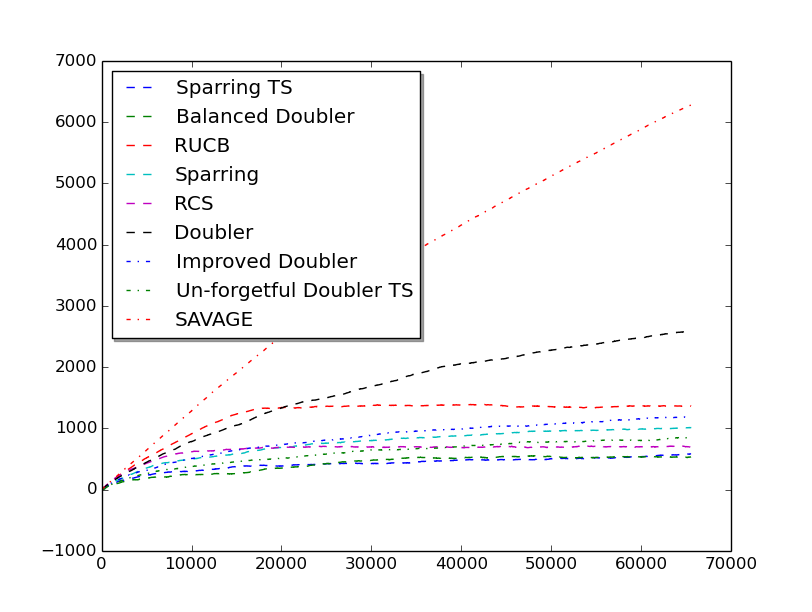
\includegraphics[scale=0.5, natwidth=610,natheight=642]{figures/all_MQ2007_7arms.png}
%  \caption{Utility Based Regret with 7 Arms}
%\end{figure}
%
%For a larger number of arms we can see that RCS and RUCB are outperformed by the other algorithms.
%
%\begin{figure}[h!]
%\centering
%  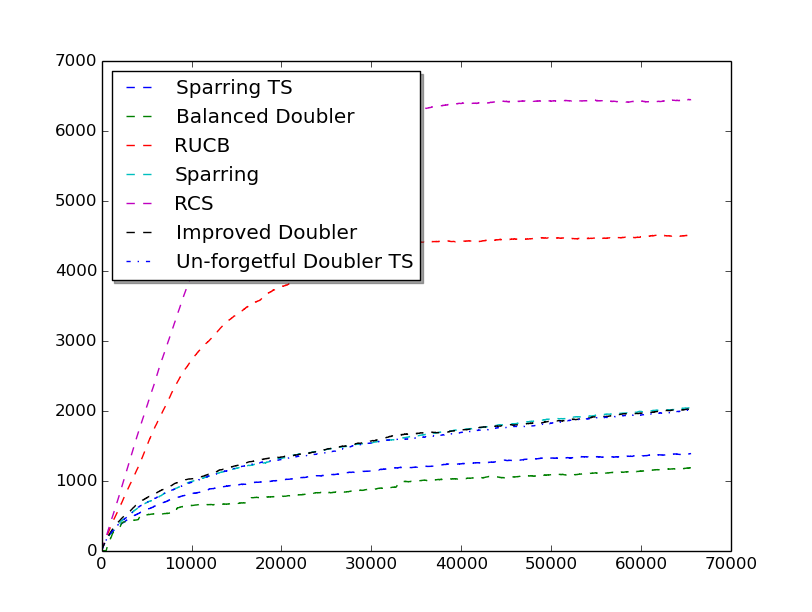
\includegraphics[scale=0.5, natwidth=610,natheight=642]{figures/all_MQ2007_24arms.png}
%  \caption{Utility Based Regret with 24 Arms}
%\end{figure}
%
%And for 46 arms we can see that Sparring with Thompson Sampling methods performs better than all the other algorithms.
%
%
%\subsection{Sparring}
%
%We can see the clear advantage of using the Sparring algorithm over the RCS algorithm when dealing with a large number of arms.
%\begin{figure}[h!]
%\centering
%\begin{subfigure}{.5\textwidth}
%  \centering
%  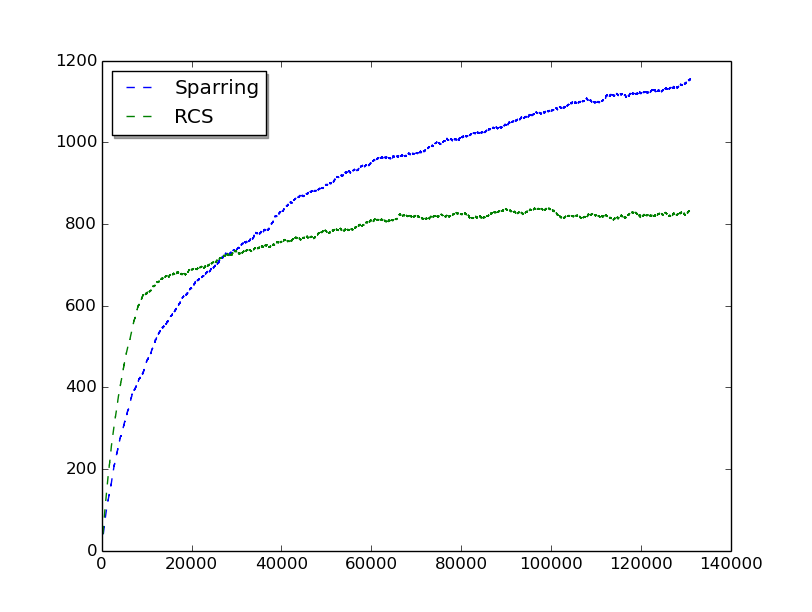
\includegraphics[scale=0.3, natwidth=410,natheight=442]{figures/rcs_sparring_MQ2007_7arms.png}
%  \caption{7 Arms}
%  \label{fig:sub1}
%\end{subfigure}%
%\begin{subfigure}{.5\textwidth}
%  \centering
%  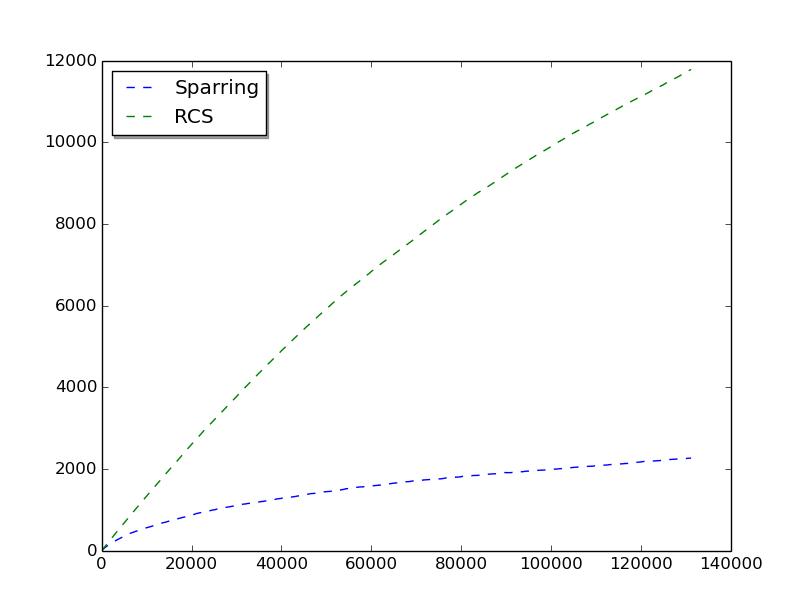
\includegraphics[scale=0.3, natwidth=410,natheight=442]{figures/rcs_sparring_MQ2007_16arms.png}
%  \caption{16 Arms}
%  \label{fig:sub2}
%\end{subfigure}
%\begin{subfigure}{.5\textwidth}
%  \centering
%  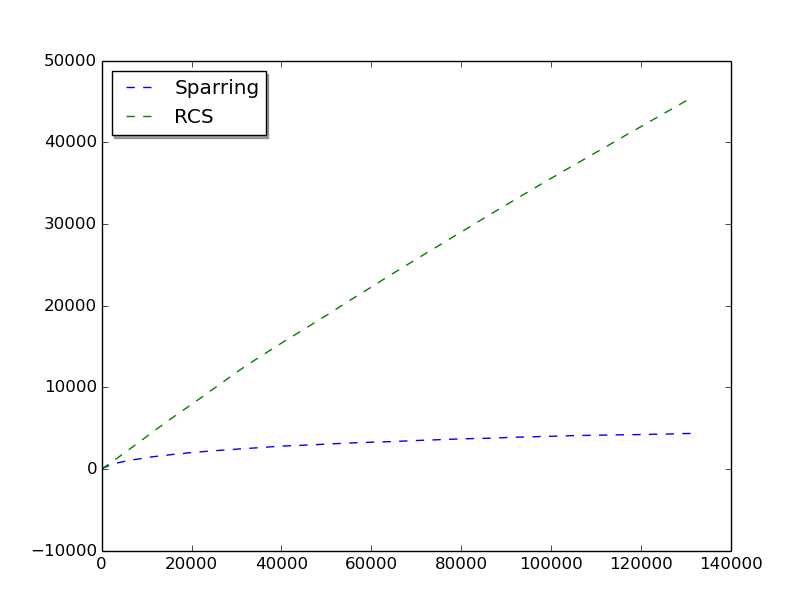
\includegraphics[scale=0.3, natwidth=410,natheight=442]{figures/rcs_sparring_MQ2007_46arms.png}
%  \caption{46 Arms}
%  \label{fig:sub2}
%\end{subfigure}
%\caption{RCS Versus Sparring with Utility Based Regret}
%\label{fig:test}
%\end{figure}
%
%
%With a small number of arms (Fig 1.) we can observe that the RCS algorithm quickly converges to the optimal arm.
%\\
%With a larger number of arms we can see that Sparring out-performs the RCS algorithm. 
%\\
%Now lets look at the general regret (as defined section 2.2). Here we used 46 arms:
%\begin{figure}[h!]
%  \centering
%     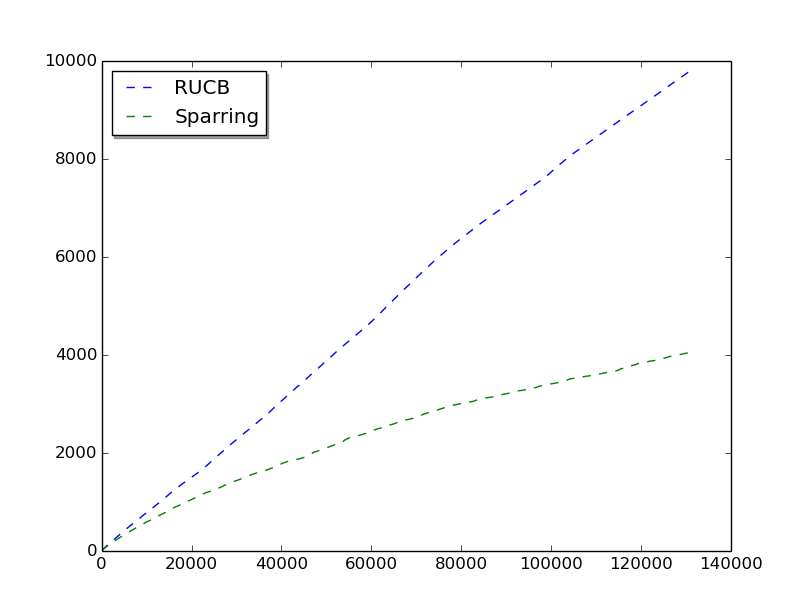
\includegraphics[scale=0.4, natwidth=410,natheight=442]{figures/rcs_sparring_MQ2007_general.png} 
%  \caption{RCS Versus Sparring with Preference Based Regret with 46 Arms}
%\end{figure}
%
%
%\newpage
%\subsection{Doubler}
%Now lets have a look at the Doubler algorithm using the same data set.
%\begin{figure}[h!]
%\centering
%\begin{subfigure}{.5\textwidth}
%  \centering
%  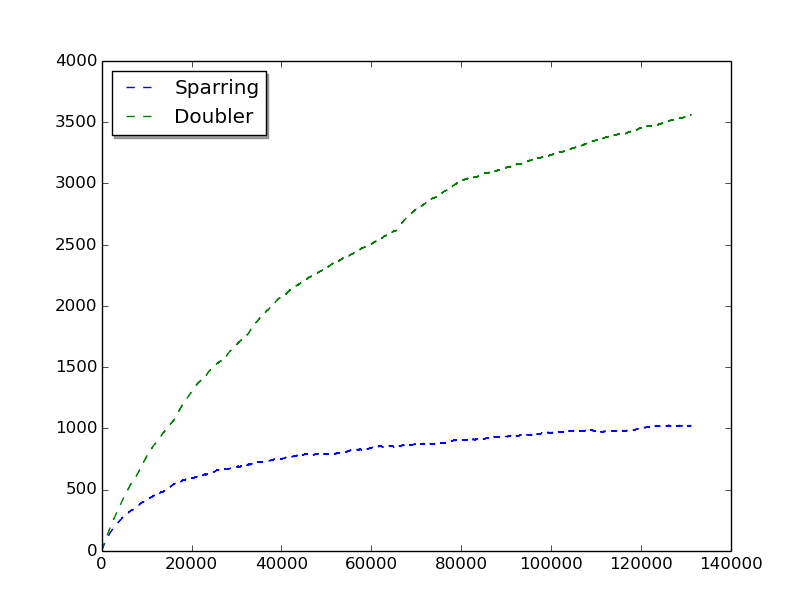
\includegraphics[scale=0.3, natwidth=410,natheight=442]{figures/doubler_sparring_MQ2007_7arms.png}
%  \caption{7 Arms}
%  \label{fig:sub1}
%\end{subfigure}%
%\begin{subfigure}{.5\textwidth}
%  \centering
%  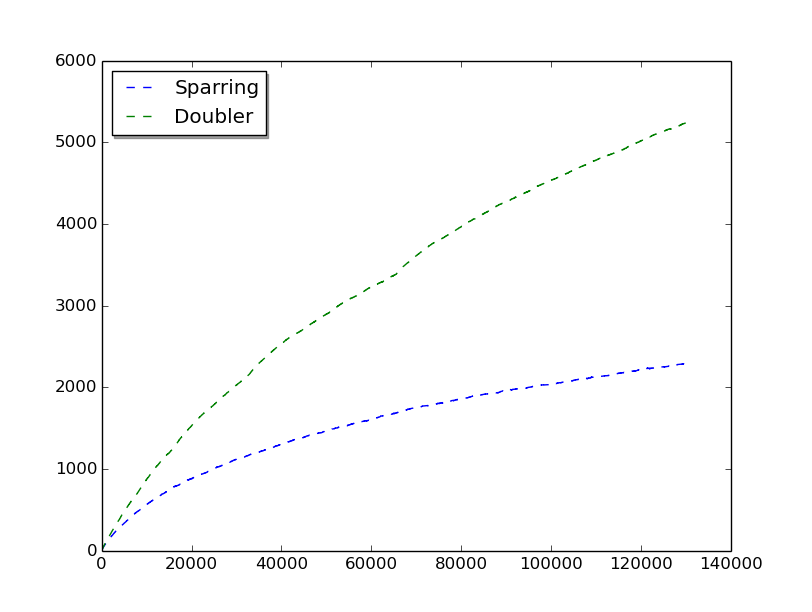
\includegraphics[scale=0.3, natwidth=410,natheight=442]{figures/doubler_sparring_MQ2007_16arms.png}
%  \caption{16 Arms}
%  \label{fig:sub2}
%\end{subfigure}
%\begin{subfigure}{.5\textwidth}
%  \centering
%  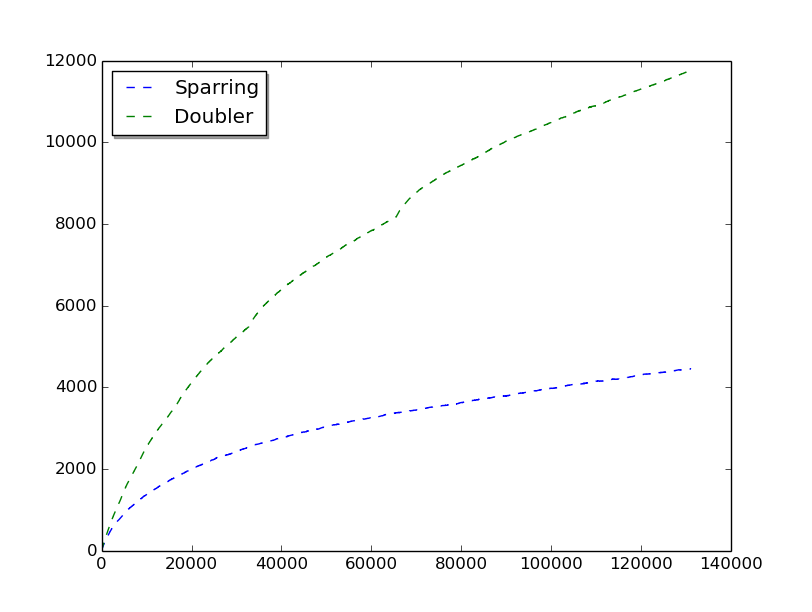
\includegraphics[scale=0.3, natwidth=410,natheight=442]{figures/doubler_sparring_MQ2007_46arms.png}
%  \caption{46 Arms}
%  \label{fig:sub2}
%\end{subfigure}
%\caption{Doubler Versus Sparring with Utility Based Regret}
%\label{fig:test}
%\end{figure}
%
%The general regret:
%\begin{figure}[h!]
%  \centering
%     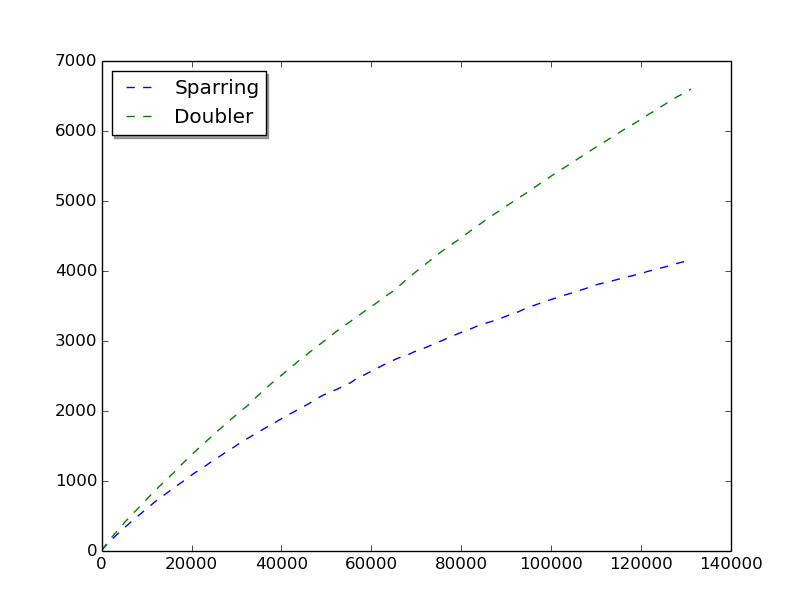
\includegraphics[scale=0.2, natwidth=410,natheight=442]{figures/doubler_sparring_MQ2007_general.png} 
%  \caption{Doubler Versus Sparring with Preference Based Regret with 46 Arms}
%\end{figure}
%
%\newpage
%\subsection{Improved Doubler}
%Now lets have a look at the Improved Doubler algorithm using the same data set.
%\begin{figure}[h!]
%\centering
%\begin{subfigure}{.5\textwidth}
%  \centering
%  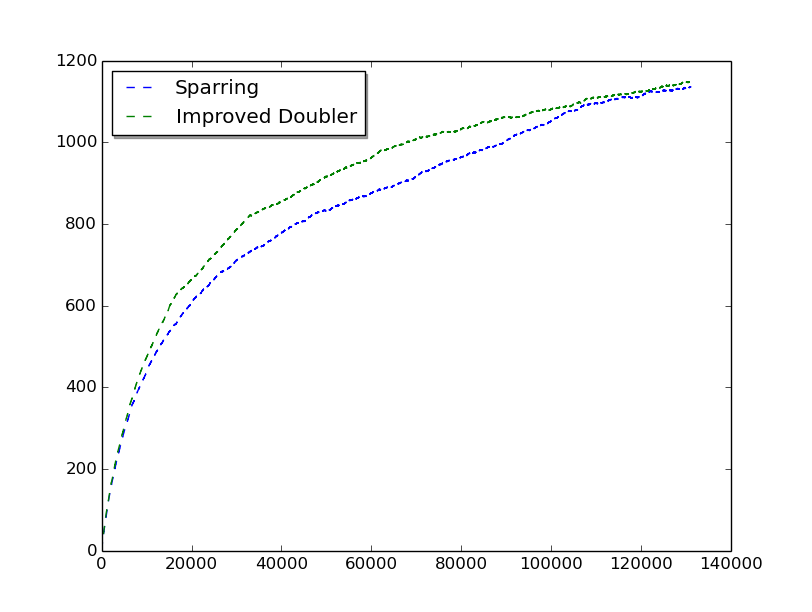
\includegraphics[scale=0.3, natwidth=410,natheight=442]{figures/improved_doubler_sparring_MQ2007_7arms.png}
%  \caption{7 Arms}
%  \label{fig:sub1}
%\end{subfigure}%
%\begin{subfigure}{.5\textwidth}
%  \centering
%  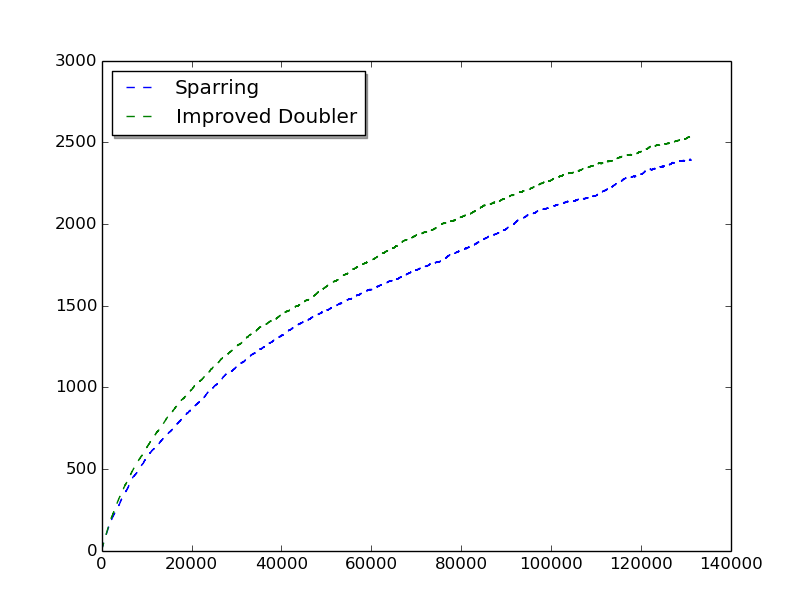
\includegraphics[scale=0.3, natwidth=410,natheight=442]{figures/improved_doubler_sparring_MQ2007_16arms.png}
%  \caption{16 Arms}
%  \label{fig:sub2}
%\end{subfigure}
%\begin{subfigure}{.5\textwidth}
%  \centering
%  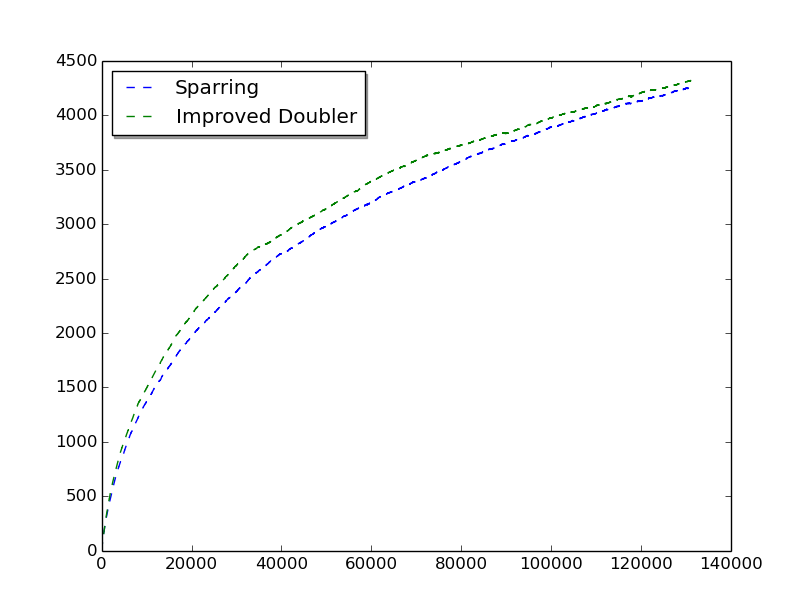
\includegraphics[scale=0.3, natwidth=410,natheight=442]{figures/improved_doubler_sparring_MQ2007_46arms.png}
%  \caption{46 Arms}
%  \label{fig:sub2}
%\end{subfigure}
%\caption{Improved Doubler Versus Sparring with Utility Based Regret}
%\label{fig:test}
%\end{figure}
%
%The general regret:
%\begin{figure}[h!]
%  \centering
%     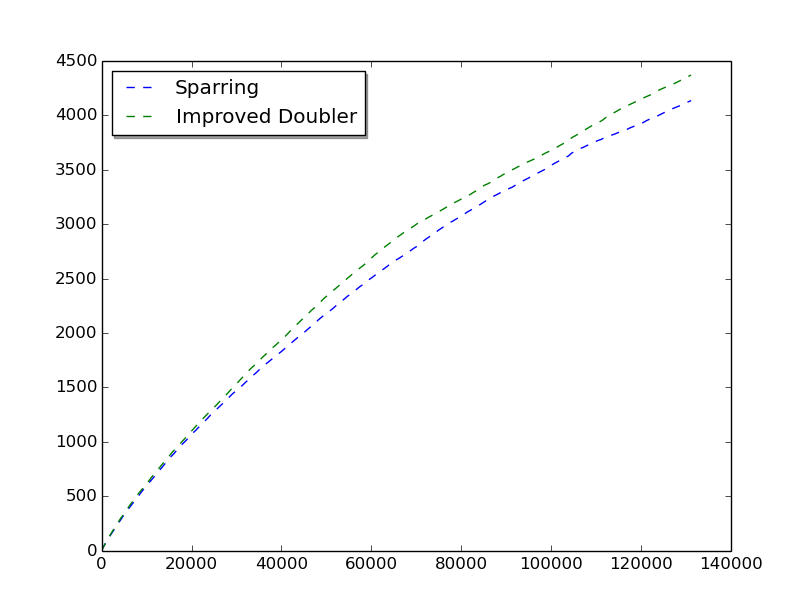
\includegraphics[scale=0.3, natwidth=410,natheight=442]{figures/improved_doubler_sparring_MQ2007_general.png} 
%  \caption{Improved Doubler Versus Sparring with Preference Based Regret with 46 Arms}
%\end{figure}
%\newpage
%\subsection{Balanced Doubler}
%Now lets have a look at the Balanced Doubler algorithm using the same data set.
%\begin{figure}[h!]
%  \centering
%     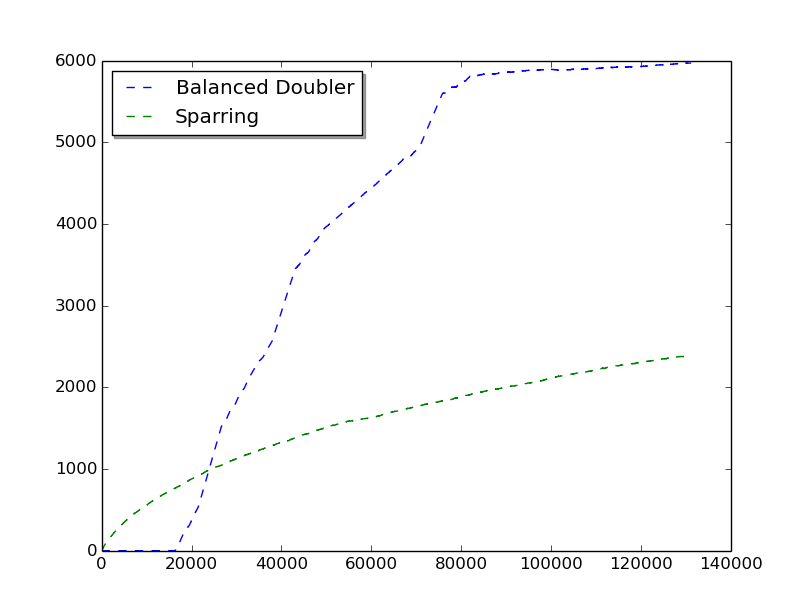
\includegraphics[scale=0.3, natwidth=410,natheight=442]{figures/balanced_doubler_sparring_MQ2007_16arms.png} 
%  \caption{Balanced Doubler Versus Sparring with Utility Based Regret with 16 Arms}
%\end{figure}
%
%\subsection{Thompson Sampling Doubler}
%Now lets have a look at the Balanced Doubler algorithm using the same data set.
%\begin{figure}[h!]
%\centering
%\begin{subfigure}{.5\textwidth}
%  \centering
%  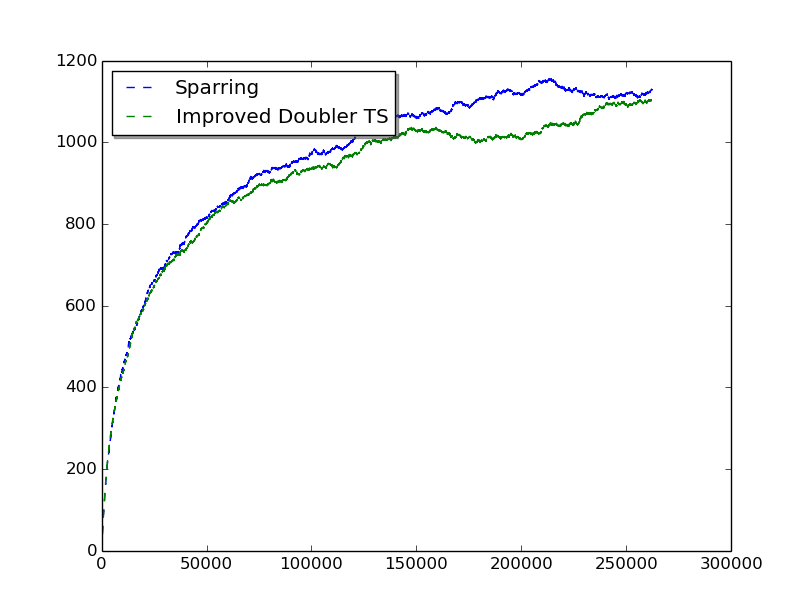
\includegraphics[scale=0.3, natwidth=410,natheight=442]{figures/improved_doubler_TS_sparring_MQ2007_7arms.png}
%  \caption{7 Arms}
%  \label{fig:sub1}
%\end{subfigure}%
%\begin{subfigure}{.5\textwidth}
%  \centering
%  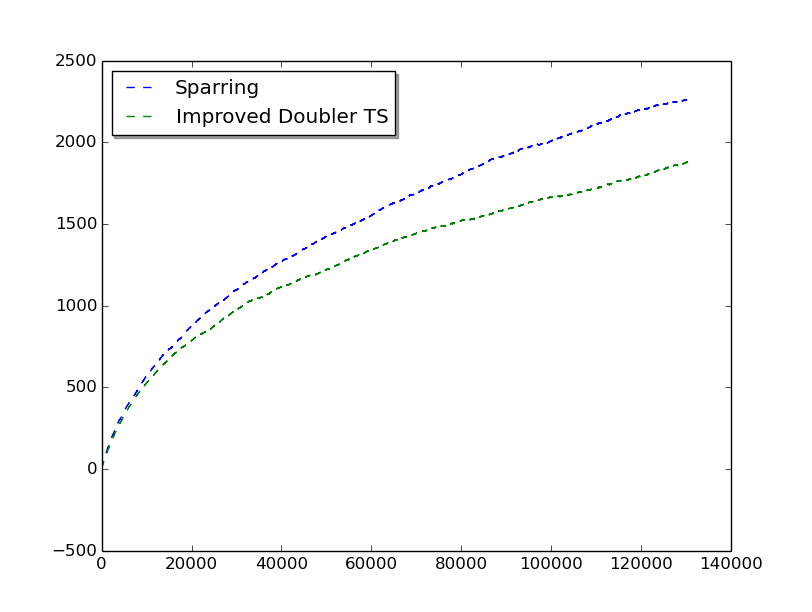
\includegraphics[scale=0.3, natwidth=410,natheight=442]{figures/improved_doubler_TS_sparring_MQ2007_16arms.png}
%  \caption{16 Arms}
%  \label{fig:sub2}
%\end{subfigure}
%\begin{subfigure}{.5\textwidth}
%  \centering
%  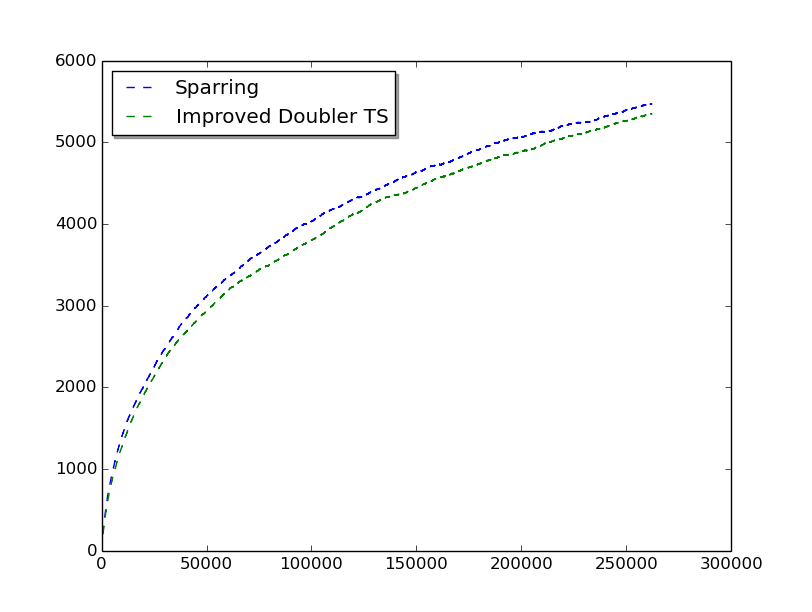
\includegraphics[scale=0.3, natwidth=410,natheight=442]{figures/improved_doubler_TS_sparring_MQ2007_46arms.png}
%  \caption{46 Arms}
%  \label{fig:sub2}
%\end{subfigure}
%\caption{Improved Doubler Versus Sparring with Utility Based Regret}
%\label{fig:test}
%\end{figure}
%
%The general regret:
%\begin{figure}[h!]
%  \centering
%     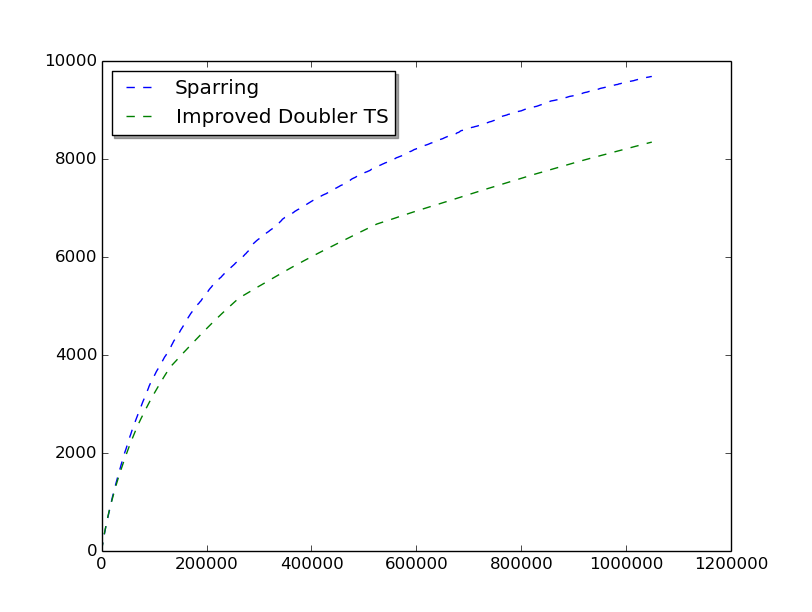
\includegraphics[scale=0.4, natwidth=410,natheight=442]{figures/improved_doubler_TS_sparring_MQ2007_general.png} 
%  \caption{Improved Doubler Versus Sparring with Preference Based Regret with 46 Arms}
%\end{figure}
%
%\subsection{Thompson Sampling Sparring}
%And finally, lets show the results of  the sparring algorithm when using Thompson Sampling black boxes.
%
%\begin{figure}[h!]
%  \centering
%     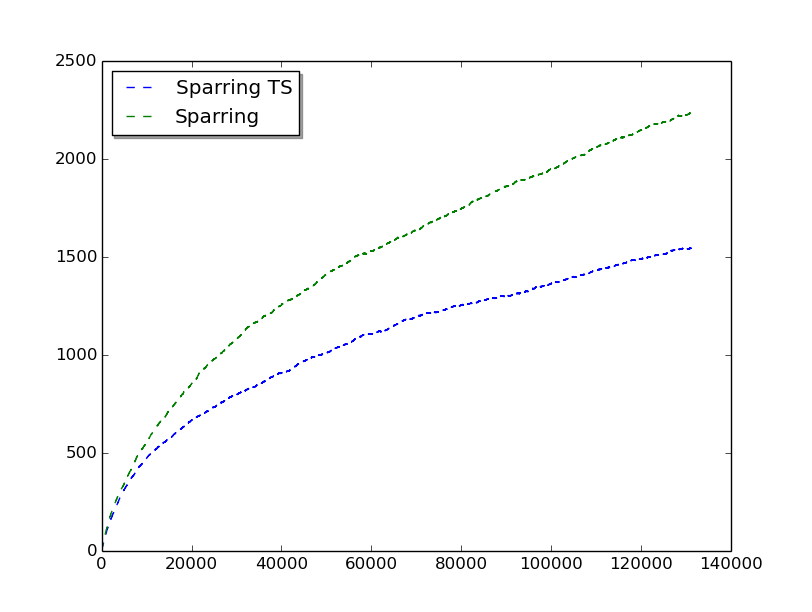
\includegraphics[scale=0.4, natwidth=410,natheight=442]{figures/TS_sparring_sparring_MQ2007_16arms.png} 
%  \caption{Thompson Sampling Sparring Versus Sparring with Utility Based Regret with 16 Arms}
%\end{figure}
%
%The general regret:
%\begin{figure}[h!]
%  \centering
%     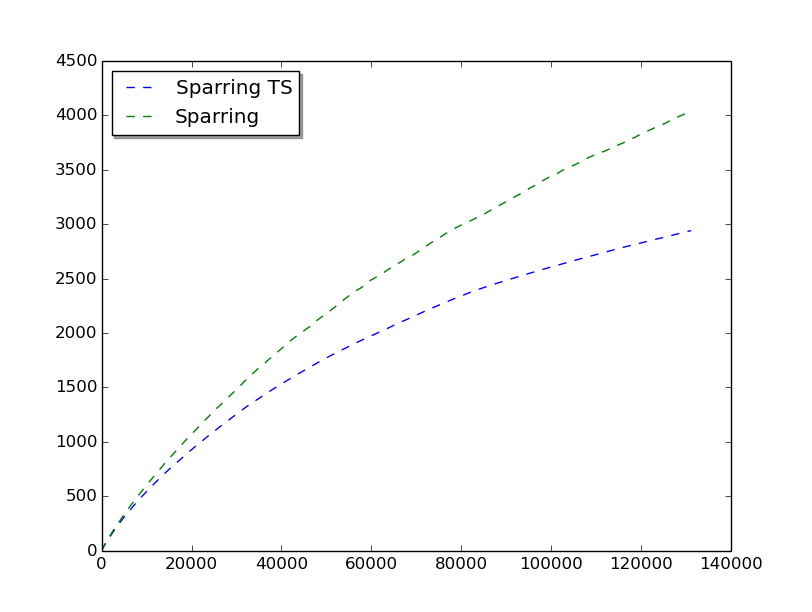
\includegraphics[scale=0.4, natwidth=410,natheight=442]{figures/TS_sparring_sparring_MQ2007_general.png} 
%  \caption{Thompson Sampling Sparring Versus Sparring with Preference Based Regret with 46 Arms}
%\end{figure}

\end{document}
